
\NewChapter{2}{2}



\counterwithin{figure}{section}

\begin{refsection}
\begin{center}
\hspace{}
\\[0.5 in]

Deep Convolutional Residual Regressive Neural Networks \\
and Sea Surface Temperatures from Aqua \& Argo in the 2000s

\\[1.0in]

Albert Eric Larson and Ali Shafqat Akanda\\[1.0in]

\emph{Submitted to MDPI Remote Sensing}
\end{center}
\newpage

\subsection{Abstract}
Sea surface temperature (SST) is an essential climate variable that can be measured via ground truth, remote sensing, or hybrid “model” methodologies. Here, we celebrate the progress of high resolution sea surface temperature via the acknowledgement of a few technological advances from the late 20th and early 21st century. Specifically, we observe three snapshots of twelve monthly SST measurements in 2010 as measured by the passive microwave radiometer AMSR-E, the visible and infrared monitoring MODIS instrument, and the in situ Argo dataset ISAS. We author simple scripts to perform the functions of an extract, transform, and load system. We experiment with a machine learning technology known as deep convolutional residual regressive neural networks and attempt to fuse AMSR-E and MODIS into a superior product. Looking forward, we hope to integrate F2F with future satellite missions such as Surface Water Ocean Topography (SWOT) or Interferometric Synthetic Aperture Radar (InSAR) to enhance the precision of coastal regions observations of water.

\subsection{Introduction}
Under the auspices of its 193 member states, the World Meteorological Organization holds of particular importance certain physical measurements of Earth and the surrounding environment. Each parameter is singled out by being promoted under the acronym ECV, denoting the physical measurement to be an Essential Climate Variable. Furthermore, the same organization has established goals and deadlines for the participating countries to sustain all forms of life on Earth, known as sustainable development goals or SDGs.

Evidence continues to mount that human beings through industrialization have modified and are continuing to significantly modify the climate. However, the modern cause for concern is the rate at which our climate has changed rather than the Boolean of has it or has it not. Measurements of carbon dioxide (CO2) tell the story: detected values of atmospheric CO2 have increased by 50\% of the starting value at the advent of industrialization (\cite{eldering2017orbiting}). Invariant to latitude and longitude, the impacts are felt everywhere. Earth’s response to our stimuli manifests in the form of heat waves, stronger storms, longer periods of drought, greater impulses of meteorological water accumulation over land, and a general increase in environmental variability. While in wealthy communities, modern civil infrastructure serves as a boundary layer to environment-related catastrophes, the poor and powerless are unequally yoked. One must consider also the importance of the ecology itself. As humanity conquers the environment, in what state are the creatures of the atmosphere, land and oceans? What does the next five, ten, five hundred years look like at the current rate? If deemed unacceptable, what changes can be made to mitigate or adapt to implications of past and present poor actions? What are the global environmental quality standards? How can standards be enforced in unequal nation states? 

There are many global environmental observation systems that study the entire Earth from a distance. The sheer volume of effort and observation output can be gleaned by world wide web crawling one example: the details of the Coupled Model Intercomparison Project website. Through this project, expert parties from all over the globe share the effort of simulating Earth by focusing on their separate silos whilst having common tunnels to assemble, communicate, benchmark, and improve. Remote sensing (RS) instruments have recently (1950 – present) grown in frequency of occurrence, capability, availability, and affordability. Attached to planes, balloons, spacecraft, or other autonomous means, these devices capture images in a controlled fashion over medium to large portions (swaths) of the land, atmosphere, and ocean. The growth of global RS data is pivotal to our ability to continuously view the macroscopic climate system. The output of these RS devices can be studied with a variety of optical techniques, in most cases altered via some logic to provide a more value-added product depending on the data consumer’s needs.  

For example, consider the delineation of processing levels provided in the peer-reviewed document coinciding with the deployment of the ECOSTRESS instrument (\cite{fisher2020ecostress}). A lower value processing level (L0, L1) indicates raw measurements of electromagnetic radiation from the Sun through Earth’s atmosphere off the land / water surface, back up to through the atmosphere to the satellite instrument. In turn, a higher value (L2 – L4) indicates the generation of physical parameters, gridding of swath data, and data assimilation with other parameters. In the instance of ECOSTRESS, the higher levels refer to land surface temperature, emissivity, measures of evapotranspiration, and at Level 4 evaporative stress and water use indices.

Here we investigate the temperature of the ocean’s surface (SST). This target is chosen because of its focus on the behavior of water in the environment, its importance in numerical weather and climate forecasting, and detectability via satellite-mounted RS instrumentation. Also, it has matched continuous ground truth temporospatial measurements that can be investigated for intercomparison of dataset bias, variances, and uncertainties. While it is not practical to grid the entire surface of Earth with sensors, in many situations and places it is extremely valuable to use arrays of dense, spatially linked precise in situ measurements. Satellite observations have a coarse resolution and can miss many interesting small-scale anomalies within the hydrosphere. 

We compare the raw satellite observations to the lower resolution but more precise measurements of sea surface temperature. We apply a treatment to the lower resolution but generally more available satellite instrument (AMSR-E), setting its target output to be the higher resolution MODIS product. Our hypothesis is that fusing the AMSR-E data to MODIS data will create a product that is closer in performance to MODIS than its AMSR-E input. 

\subsection{Materials \& Methods}
\subsubsection{Sea Surface Temperature (SST)}
The origin of SST as a continuously monitored variable began when Benjamin Franklin captured measurements of the ocean as he traversed the Atlantic, acquiring data and synthesizing these observations into information about the Gulf Stream. There is a rich history from that point forward to the present day, and a thorough review available in the literature (\cite{minnett2019half}).

SST is largely academically segregated into the field of physical oceanography. Nevertheless, the connection between ocean, atmosphere, and land are intimately intertwined. There is a trickling down from global SST anomalies like the El-Niño Southern Oscillation, the Madden Julian Oscillation, the Atlantic meridional overturning circulation, western boundary currents, gyres, and eddies to the availability of food, energy, and clean drinking water. Consequently, better understanding and application of oceanic parameters in consideration of land-based hydrology means improved forecasting and preparation for the future. 

\subsubsection{Aqua}
The Aqua satellite was launched on May 4, 2002 (\cite{parkinson2003aqua}). Upon it, two instruments sit: AMSR-E and MODIS. Both, among other things, are designed to study the temperature of the ocean. The measurements obtained as the satellite is moving from South Pole towards North always crosses the equator at approximately 1:30 PM local time nadir (directly below the satellite). In the downward portion of the orbit, the satellite crosses the equator at 1:30 AM local time nadir. 

\subsubsection{AMSR-E}
AMSR-E is a passive microwave radiometer (\cite{kawanishi2003advanced}). The acronym stands for Advanced Microwave Scanning Radiometer for Earth Observing System. There are several products produced on top of the raw radiance data collected by this instrument, and the AMSR-E data is processed by different ground stations depending on the parameter of interest. The produced datasets contain latitude, longitude, several physical parameters (e.g., SST, Albedo, soil moisture) as well as other pertinent metadata. As it pertains to sea surface temperature, AMSR-E is available in Level 2 or Level 3 products, and as part of Level 4 assimilation system output. 

To detail a sample, one single Level 2 netCDF (.nc) file containing AMSR-E data was downloaded. The record selected is that of March 3rd, 2004, with a UTC time of 01:07:01. The file contains three coordinates (latitude, longitude, and time) and thirteen data variables.

Each variable is a single matrix comprised of columns and rows of measurements. The important distinction here is that the data structure is stored to reflect the path of the orbit. See Figure \ref{fig2_1}. When the sea surface temperature is plotted as it sits in the matrix, it is difficult to discern what is transpiring. There appears to be some curvature of the measurements, but other than that little is known to an untrained eye beyond the title and colormap.

Inclusion of the latitude and longitude coordinates, as well as a global basemap generates a clearer picture as seen in Figure \ref{fig2_2}. A single Level 2 AMSR-E SST file contains matrices representing one full orbit around the globe. Each file holds partially daytime and partially nighttime observations. Because of diurnal warming, it is desirable to separate the nighttime and daytime passes. Furthermore, many analyses are comprised of an ensemble of satellite observations from different platforms such as this one. A grid makes for more orderly computations at large spatial scales. Certainly, one could elect to grid every observation to the AMSR-E or MODIS native product coordinate system. With our experiments, we choose the path of rectangular gridding. We consider the Level 3 product because of the interest in spatial relationship across large geographic scales and variable time (daily, weekly, seasonally, yearly, generationally). 

The Level 3 equidistant rectangular gridded product is accessed via the NASA Jet Propulsion Laboratory’s Physical Oceanography Distributed Active Archive Center (PODAAC) and was produced by Remote Sensing Systems of Santa Rosa, California. This product comes in 25 km resolution and is delineated by daytime and nighttime passes of the satellite. The time series runs from June of 2002 until October of 2011 when the AMSR-E instrument ceased functioning. Figure \ref{fig2_3} illustrates the point that even without explicitly defining the coordinate system in the visualization, the matrix of SST values is already placed in proper spatial order. Figure \ref{fig2_4} reinforces the fact that little change occurs with the inclusion of latitude and longitude coordinates when plotted on a rectangular grid.

We accumulate the daily daytime and nighttime readings from AMSR-E into monthly products. While a monthly product has already been produced for use with the Climate Model Intercomparison Project, AMSR-E\_CMIP5 as available from the does not delineate between daytime and nighttime. Here, we simply compute the monthly average for daytime and nighttime passes on a pixel-wise basis for each month. We finally re-grid the AMSR-E data to the MODIS L3 grid. 

\subsubsection{MODIS}
MODIS, or Moderate Resolution Imaging Spectroradiometer, measures thirty-six different radiance bands in the infrared and visible ranges of the electromagnetic spectrum (\cite{esaias1998overview}). Level 3 sea surface skin temperature as obtained from MODIS comes in 4 kilometer and 9 km products, and is derived from a subset of the thirty-six radiance bands. The products are available in daily, average of eight days, and monthly products. They are also delineated by daytime and nighttime passes of the Aqua’s polar-orbiting nature. SST products deriving from MODIS are further specified by the length of the waves within the thermal infrared range used to derive the measurement: longer waves (11–12 microns) and middling waves (3–4 microns). The MODIS documentation state that the 3–4 micron wave SST product is less uncertain, but only usable at night because of the daytime sun glint impact on 3–4 micron waves. We use the long wave 11–12 micron infrared measurements to keep constant the source of both daytime and nighttime passes.

The MODIS Aqua Level 3 SST Thermal IR Monthly 4km V2019.0 product comes with latitude and longitude coordinates, SST values and per pixel quality measurements denoting when contamination is likely. The grid is equidistant rectangular, a match with the AMSR-E grid but at a finer original resolution. Of the over thirty million pixels for an entire day of 4 km MODIS pixels, 90\% of them in the random sample selected here are deemed contaminated and filtered out (Figure \ref{fig2_5}). This contrasts with the 50\% loss of AMSR-E pixels. This great loss in pixels due to quality is attributed to cloud contamination. To compensate, we use the monthly product (Figure \ref{fig2_6}) where a greater amount of time has transpired, allowing for a higher probability of clean global coverage. A randomly sampled MODIS monthly image yields 50\% loss, in line with the AMSR-E daily product and much improved upon relative to the daily MODIS observation files.

\subsubsection{Ground Truth Measurements}
For a source of ground truth data, we selected the “In Situ Analysis System” (ISAS) dataset obtained from the University of California’s Argo repository and produced by a consortium of French institutions (\cite{gaillard2016situ}). An important constraint for this work was to obtain only the surface level measurement of temperature at the highest frequency available during the years of both AMSR-E and MODIS. These products are provided in a gridded format are used to observe temperature measurements at many depth levels. In the publication attached to the ISAS dataset (\cite{gaillard2016situ}), the target physical quantity is steric height and ocean heat content; with these as their target output, gridded depth-dependent temperature is stored as a byproduct. The 0.5 degree monthly dataset is presented in a Mercator projection, slightly different than the AMSR-E and MODIS grids. Mercator lines of longitude have a uniform distance in between them; the distance between latitudes from the equator changes. Identical to AMSR-E, we re-grid this data to the MODIS grid and coordinate system.

\subsubsection{Treatment}
The treatments we apply to the data are several configurations of one common concept: neural networks. Neural networks are not new, but the growth of graphical processing units (hardware) has enabled them to flourish in software. Neural networks are a type of learned representation. A structure is fed connected input and target pairs. Based on the predictive quality of the initial network structure, an error between the neural network output and the target occurs. This error is in turn fed to an optimization algorithm that iteratively and slightly alters each “neuron” of the initial network structure until it reaches a designated optimal state. Via many small calculations and the simultaneous application of statistical mechanics, neural networks are known to provide qualities like that of a brain, such as capturing spatial eccentricities and temporal changes in sets of related images. Neural networks are applied to a range of tasks from the more mundane such as learning a quadratic equation, to the more cutting edge, like extreme event forecasting or cancer detection. 

Transfer learning has become commonplace in the field of machine learning (\cite{weiss2016survey}). Transfer learning places an emphasis on creating reusable treatment structures for others to build on top of without inadvertently causing the audience to get lost in possibly unimportant details. We employ transfer learning to create a complex configuration with a relatively short learning curve. The neural network is characteristically deep, convolutional, residual, and regressive. Our construct is inspired by the work of residual networks (\cite{he2016deep}). However, our problem is one of a regressive nature. Sea surface temperature has a continuous temperature range that it exists within. This is a notable difference to some of the more common introductory neural network examples, such as those associated with the MNIST and CIFAR datasets where the number of possible outputs is very small (\cite{xiao2017fashion}; \cite{krizhevsky2010convolutional}). Loss functions associated with regressive problems are constrained to just a couple: mean absolute error (MAE) and mean squared error (MSE). The calculation of the loss function must be differentiable. This is due to the optimization component of neural networks. The literature is rich with publications regarding neural network optimizers, as well as the general mechanics of neural nets (\cite{andrychowicz2016learning}; \cite{kingma2014adam}).

Once neural network architecture and hyperparameters are chosen, training and validation data is loaded into the network. While training the neural network, close observation is made of the reduction in error between training input and output as the neural network begins to optimize or learn. We also monitor the validation dataset at each training iteration. The learning process stops once the training and validation data has been passed through the network a certain number of times, or epochs. When prototyping or pilot-testing the experiment set to be carried out, one should test with a very short number of epochs and a larger sum of epochs to see where good performance meets fast time of computation.  

After training, the optimized neural network structure is intentionally frozen. Before the point of freezing, the neurons of the network can be adjusted for optimization, like a student asking a teacher for advice when studying. The frozen state and inference imposed upon it is like a student being prompted with a pop quiz and no teacher assistance. This test or input data are similar enough to the training that the teacher believes the student will have success in passing the test according to the selected merit (mean squared error, the loss function). After the test, the performance of the model is evaluated and a decision is made regarding next logical steps in the research.

A neural network can become biased to its training inputs. It starts to memorize the training dataset, which does not make for a generally applicable algorithm. Avoidance of biasing comes at the cost of variance (\cite{geman1992neural}). Applying dropout is one technique to systematically prevent system bias by simply “turning off” a certain percentage of random neurons at each iteration of the algorithm (\cite{hinton2012improving}; \cite{srivastava2014dropout}). Another approach is the application of early stopping. The loss function of a neural network typically looks like a very steep curve down to a flat bottom. Rather than allow the network to persist in the flat bottom for long and become overfit, simple logic can be employed to stop training early when the network shows evidence that it has reached an optimal state. Percentage of data split between training and testing proportions is another relevant training hyperparameter. A larger proportion of the dataset being part of the training portion could lead to overfitting of the model and lack of generalized predictability. On the other hand, insufficient training data might lead to an inability to adequately characterize the reality of the data pairs.

The image sets subjected to treatment are on the large side computationally. Holding many one million or nine million pixel images within the memory of a single graphical processing unit becomes intolerable to the device. One could elect to use multiple GPUs or a compute node with a great provision of memory. Here, we constrain the experiment to a single GPU and cut the images up into smaller pieces of square data. Our patch size is fixed at 100 x 100, though this is a tunable hyperparameter. Figure \ref{fig2_7} shows a Pacific Ocean study region, highlighting Hawaii and regions east. While this image is too large to process directly in the neural network, we can solve this problem by creating the eighteen patches of 100 x 100 pixels, representing the 300 x 600 pixel region under observation. 

Neural networks do not function when nan values are present in any of the images. We enacted a broad treatment to the AMSR-E and MODIS images, computing the mean of the entire image, excluding the nan values. Then, where the nan values are present, we replace them with the mean value. This has the convenient byproduct of introducing into the neural network many training pairs where the input and output are simply comprised of the average global SST value as obtained via the AMSR-E and MODIS instrument.

\subsection{Results}
We prepared the SST data for nine different cases all studying the year 2010: the \textbf{A}tlantic, \textbf{P}acific, and \textbf{I}ndian Oceans segmented by monthly \textbf{D}ay, \textbf{N}ight, and \textbf{H}ybrid (nb, hybrid means day and night images averaged together) observations of SST (nb, first letters of the previous are bolded to call attention for their use in Figure \ref{fig2_8}). We train the neural network on the first ten months of the year, validate with the eleventh month, and test with the twelfth month. A training session runs for 100 epochs. Each image in the geographically constrained time series is 300 pixels x 600 pixels in size, divided up into eighteen 100 x 100 pixel segments to incrementally feed the neural net.

In all instances, both training and validation loss functions drop by several orders, indicating successful training without overparameterization as would be indicated by low training error but high validation error. Performance of network as it relates to the test data, December 2010, is seen in the upper plot of Figure \ref{fig2_8}. The goal is for measurements labeled Pred or Optim to bring the RMSE value between AMSR-E and Argo or MODIS down. Pred is the prediction directly from the neural network. The Optim case takes the Pred and performs a band pass on the signal. If there are any measurements outside three standard deviations of the mean, they are replaced with nan values instead. This is a device meant to combat some of the challenges with coastal artifact.

In every case, the RMSE between the optim and MODIS is higher than the AMSR-E input. In some instances, the test case of December does make an optim output that is closer to Argo than the input AMSR-E. In some cases, though, it makes a worse performing product with regards to Argo than either AMSR-E or MODIS. A bright spot is that the optim output is closer to MODIS than the Argo product. See Figures \ref{fig2_9} and \ref{fig2_10} for samples of how the RMSE translates to actual transformation of the images.  

\subsection{Discussion}
While the continual development of a relatively open extract, transform, and load (\cite{bansal2015integrating}) system along with creation of the actual destination for the loaded data (namely the neural network treatment and posttest analytics) is certainly a plus, the results of this study request future engagement. In every case of this study, the neural network appears to struggle with coastal regions. This is due to the nature of the land sea boundary layer in all these datasets. At the presence of land, the raw data (as they are downloaded as .nc files) are given a non-number (nan) designation. Neural networks weren’t designed optimally for the currently produced segregated RS datasets. The datasets appear to be manufactured with the understanding that one group of people are still more interested in ocean behaviors, another land behavior. For the purpose of training a neural network using the convolutional flavor, images with no nans are needed. As referenced earlier, steps were taken during the training process to circumvent the presence of land by substituting those pixels temporarily with the local mean value. Another option is the application of the substitution of the nan values with the mean as computed by the entire “scene” or day. There is the potential and a likelihood that the substitution of these values is introducing a source of structured noise. This noise might be leading to the higher than preferable test performance as denoted in Figure \ref{fig2_8}. Furthermore, it is probable that this structured noise is hindering training of the neural network process itself. 

As it relates to computer vision tasks such as this set of experiments, the use of mean squared error as a loss function has been called into question as an appropriate target (\cite{wang2009mean}). Their results certainly warrant some concern, and our experiments have some corroboration with their findings. Our images are single channel inputs and can be considered grayscale pictures. When displaying SST images, we use a colormap based on what we know to be the physical limits of the parameter itself. This is a different approach than typical of image based machine learning techniques. Alternate loss functions to the standards baked into PyTorch are available (\cite{kastryulin2022image}). These functions require the inputs to be either between 0 and 1 (grayscale) or 0 and 255 (color images). Another avenue is the pursuit of physics-based loss functions (\cite{psaros2022meta}). While neural networks are a useful tool, they alone are not a silver bullet, especially as it relates to geophysics. However, the neural network community has a keen interest in computational efficiency.

We applied a land mask generated from the MODIS instrument. Aqua has far surpassed its projected useful life span and was designed before the new millennium. The new Surface Water Ocean Topography (SWOT) mission launched in 2023 (\cite{fu2009swot}; \cite{morrow2019global}). It will bring many new insights to the hydrology community. Among those insights are a more precise global picture of Earth’s coastal regions. 

Only a fraction of the available data was observed in this study. The ISAS Argo dataset was a single file attached to a DOI address of over fifty gigabytes. We extracted simple the surface layer of this dataset. There is great value in consideration of SST depth layers. Furthermore, we studied monthly time series images of all three raw datasets. AMSR-E and MODIS each have near complete global pictures within two to three days. These datasets are then transformed in different ways and can lose fidelity by various types of decimation such as regridding from swaths to squares, uncertainty in formulas used for conversion from base input to high level (L2 - L4) physical parameter, or by forms of compression. 

Cloud cover is a persistent factor at play within the community. The question of “is the measurement (pixel) currently observed impacted in an undetectable way?” can’t fully go away, because even at the hyperlocal “nowcasting” time scale there is missed detection of events. Because of the pervasive challenges, people need to come together. Great global solutions require more cooperation, engagement, and the act of building bridges with one another. Missions like the International Space Station, Artemis, Landsat, and GRACE, and SWOT are only examples of what global cooperation can result in. Here at the microscopic level of single parameter consideration, we need more of the same type of teamwork. Dynamic collaboration amongst many stakeholders raises economic efficiencies. Improvement of just a single ECV requires takes the participation of a deep supply chain. Water is life. It connects the global ecosystem in nearly every facet, from food supplies, health of exotic wild animals, to the manufacturing of semiconductor chips and the treatment of industrial water. A clearer perspective is always welcomed to help sustain life. The missions of Aqua and Argo certainly achieved their planned missions in that way.

\subsection{Conclusion}
Sea surface temperature is an essential climate variable and crucial to understand the movement of water throughout the hydrosphere. The beginning of the 21st century marked a new frontier in the measurement of SST via the Aqua mission and Argo program. We observed three overlapping datasets focused on measurements of sea surface temperature: AMSR-E microwave measurements, MODIS infrared measurements, and ISAS Argo float in situ measurements. We focus the study on three large oceanic regions: Indian, Pacific, and Atlantic. We used Flux to Flow, an extract, transform, load, treat, and evaluation framework based around a deep convolutional residual regressive neural network. We attempt to transform the coarser resolution satellite product towards the finer one and intercompare all datasets. While the neural network performs well according to its typical loss functions, we find that the presence of frequent nan values, the limitations of mean squared error as a loss function used in computer vision tasks, and the sheer size of output target quantities compounded with high desired precision results in limited success when applying the neural network transformation. We see the future of this framework including other treatment algorithms, experiments where fewer output target values are considered, or computing resources run in tandem to build a bigger network for a potential better grasp on the transformation process. 

\newpage
\subsection{Code Availability}
Scripts are available at \url{https://github.com/albertlarson/f2f_sst}

\subsection{References}
\printbibliography[heading=none]
\end{refsection}

\newpage
\subsection{Appendix}
\begin{figure}[!ht]
	\centering
    \caption{L2 AMSR-E SST field, March 3, 2004, no coordinate system}
	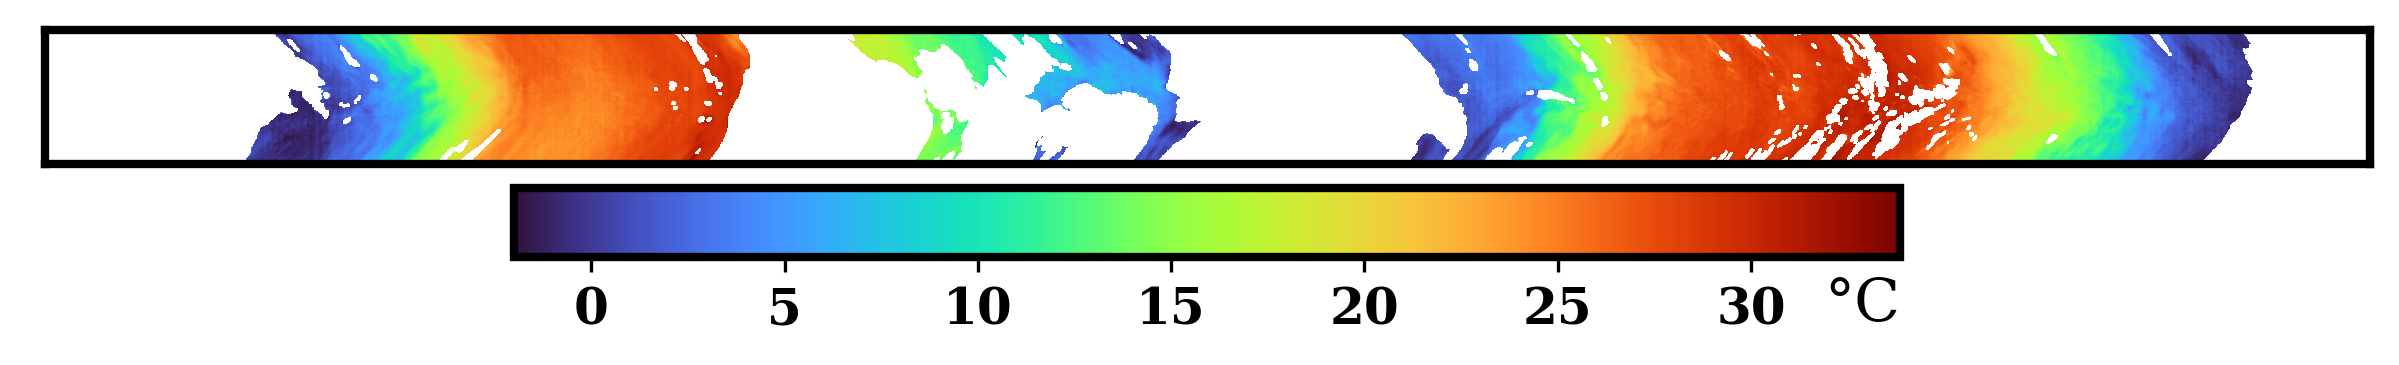
\includegraphics[width=1.0\linewidth]{m2/ims/fig2_1.png}
    \label{fig2_1}
\end{figure}

\begin{figure}[!ht]
	\centering
    \caption{L2 AMSR-E SST, plotted with available coordinates and world map}
	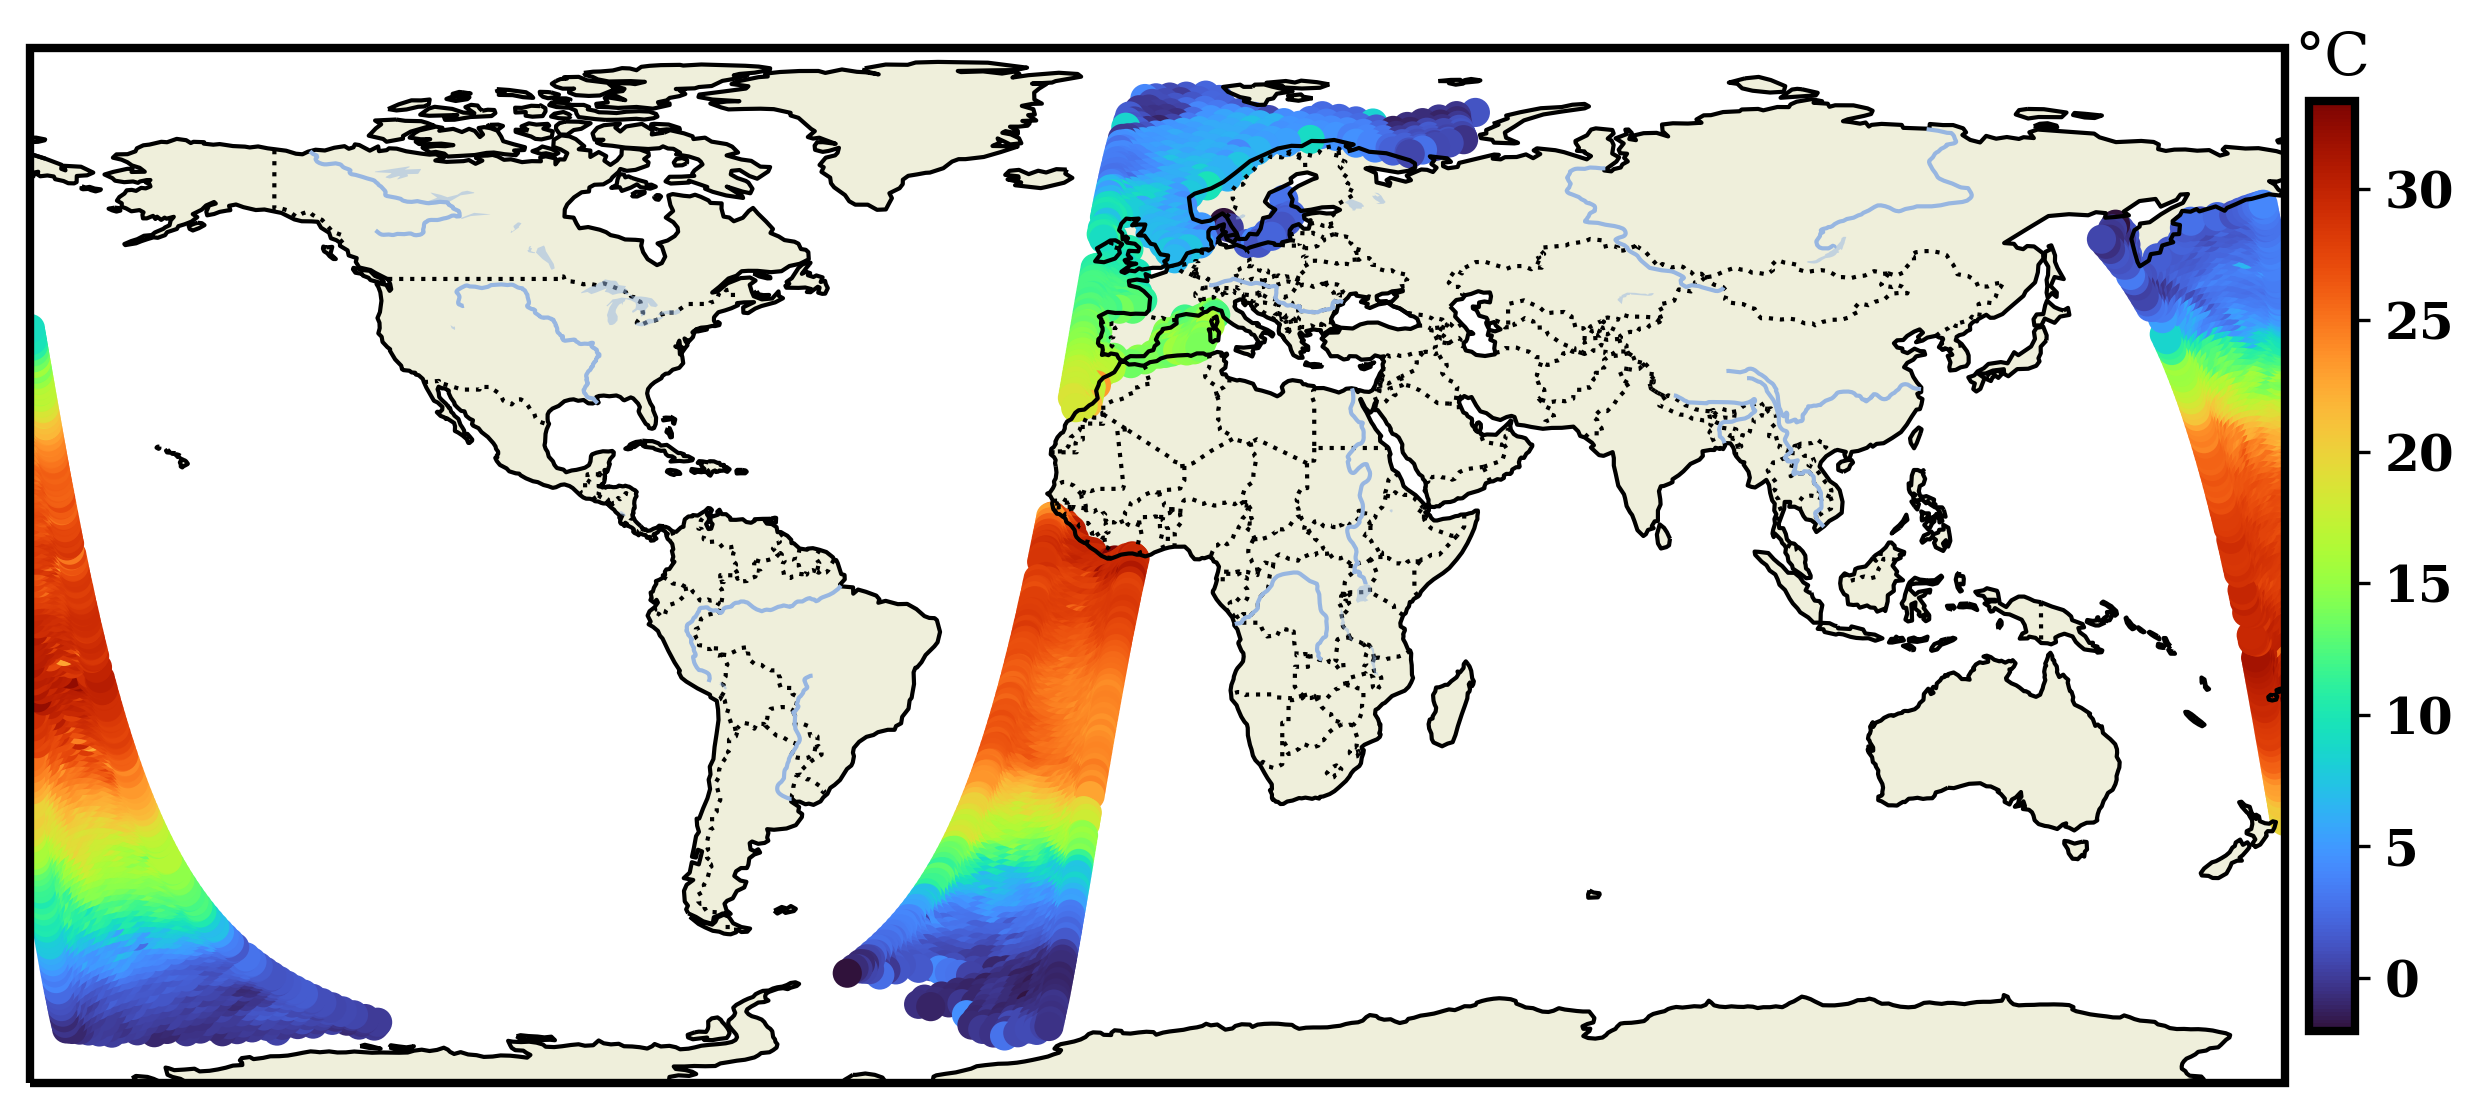
\includegraphics[width=1.0\linewidth]{m2/ims/fig2_2.png}
    \label{fig2_2}
\end{figure}

\begin{figure}[!ht]
	\centering
    \caption{L3 AMSR-E file plotted without supplied coordinate system}
	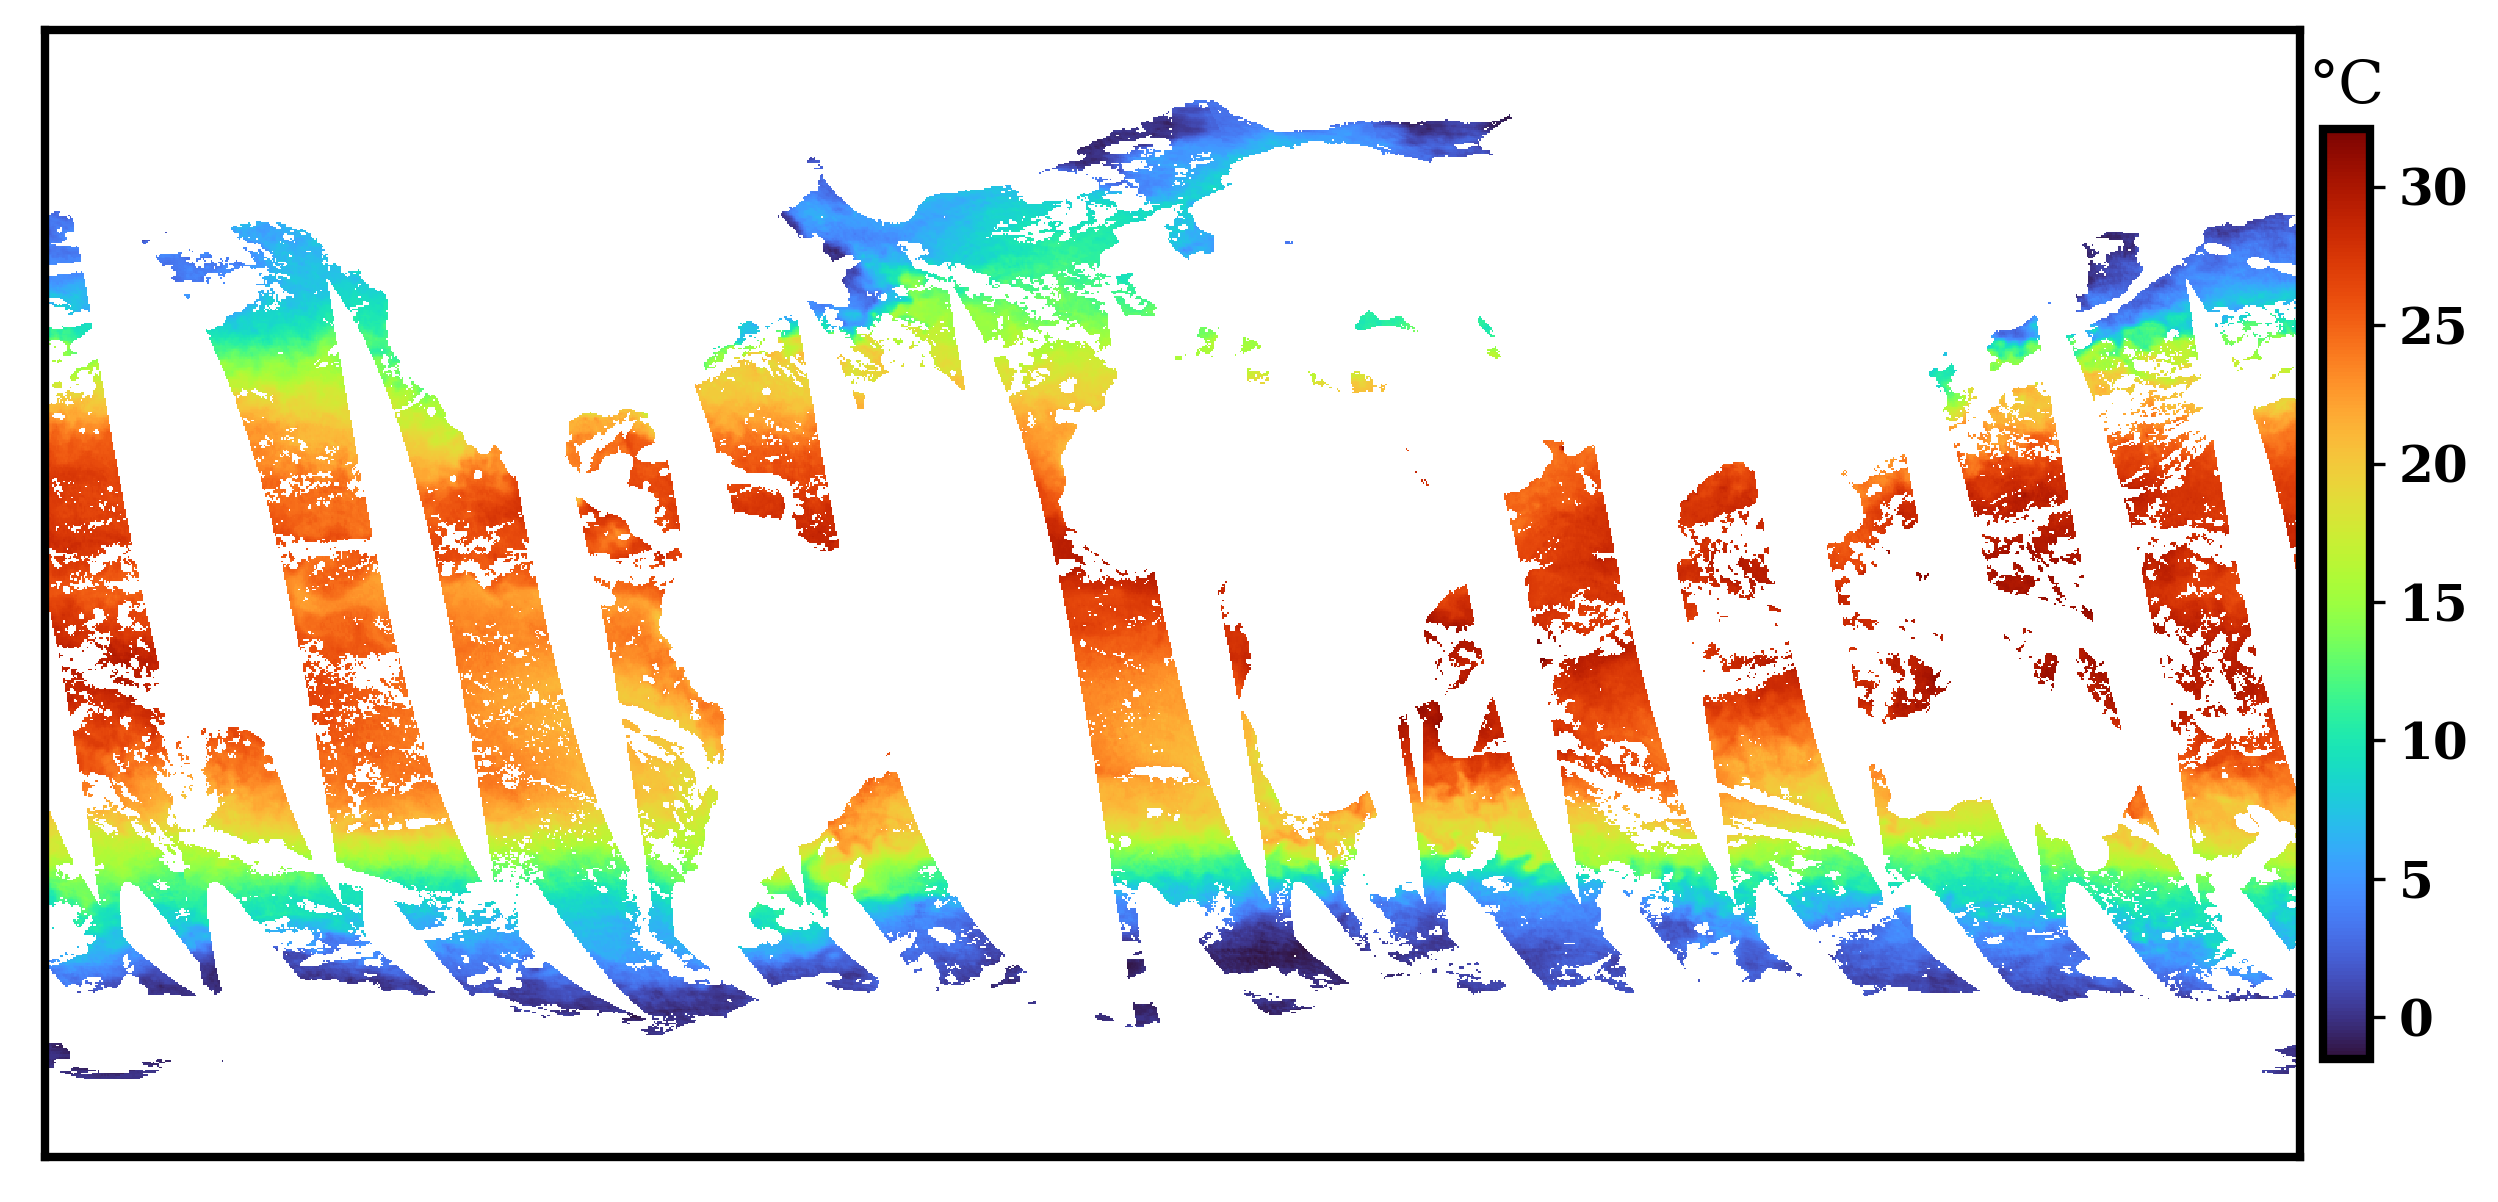
\includegraphics[width=1.0\linewidth]{m2/ims/fig2_3.png}
    \label{fig2_3}
\end{figure}

\begin{figure}[!ht]
	\centering
    \caption{L3 AMSR-E file plotted with available coordinates and world map}
	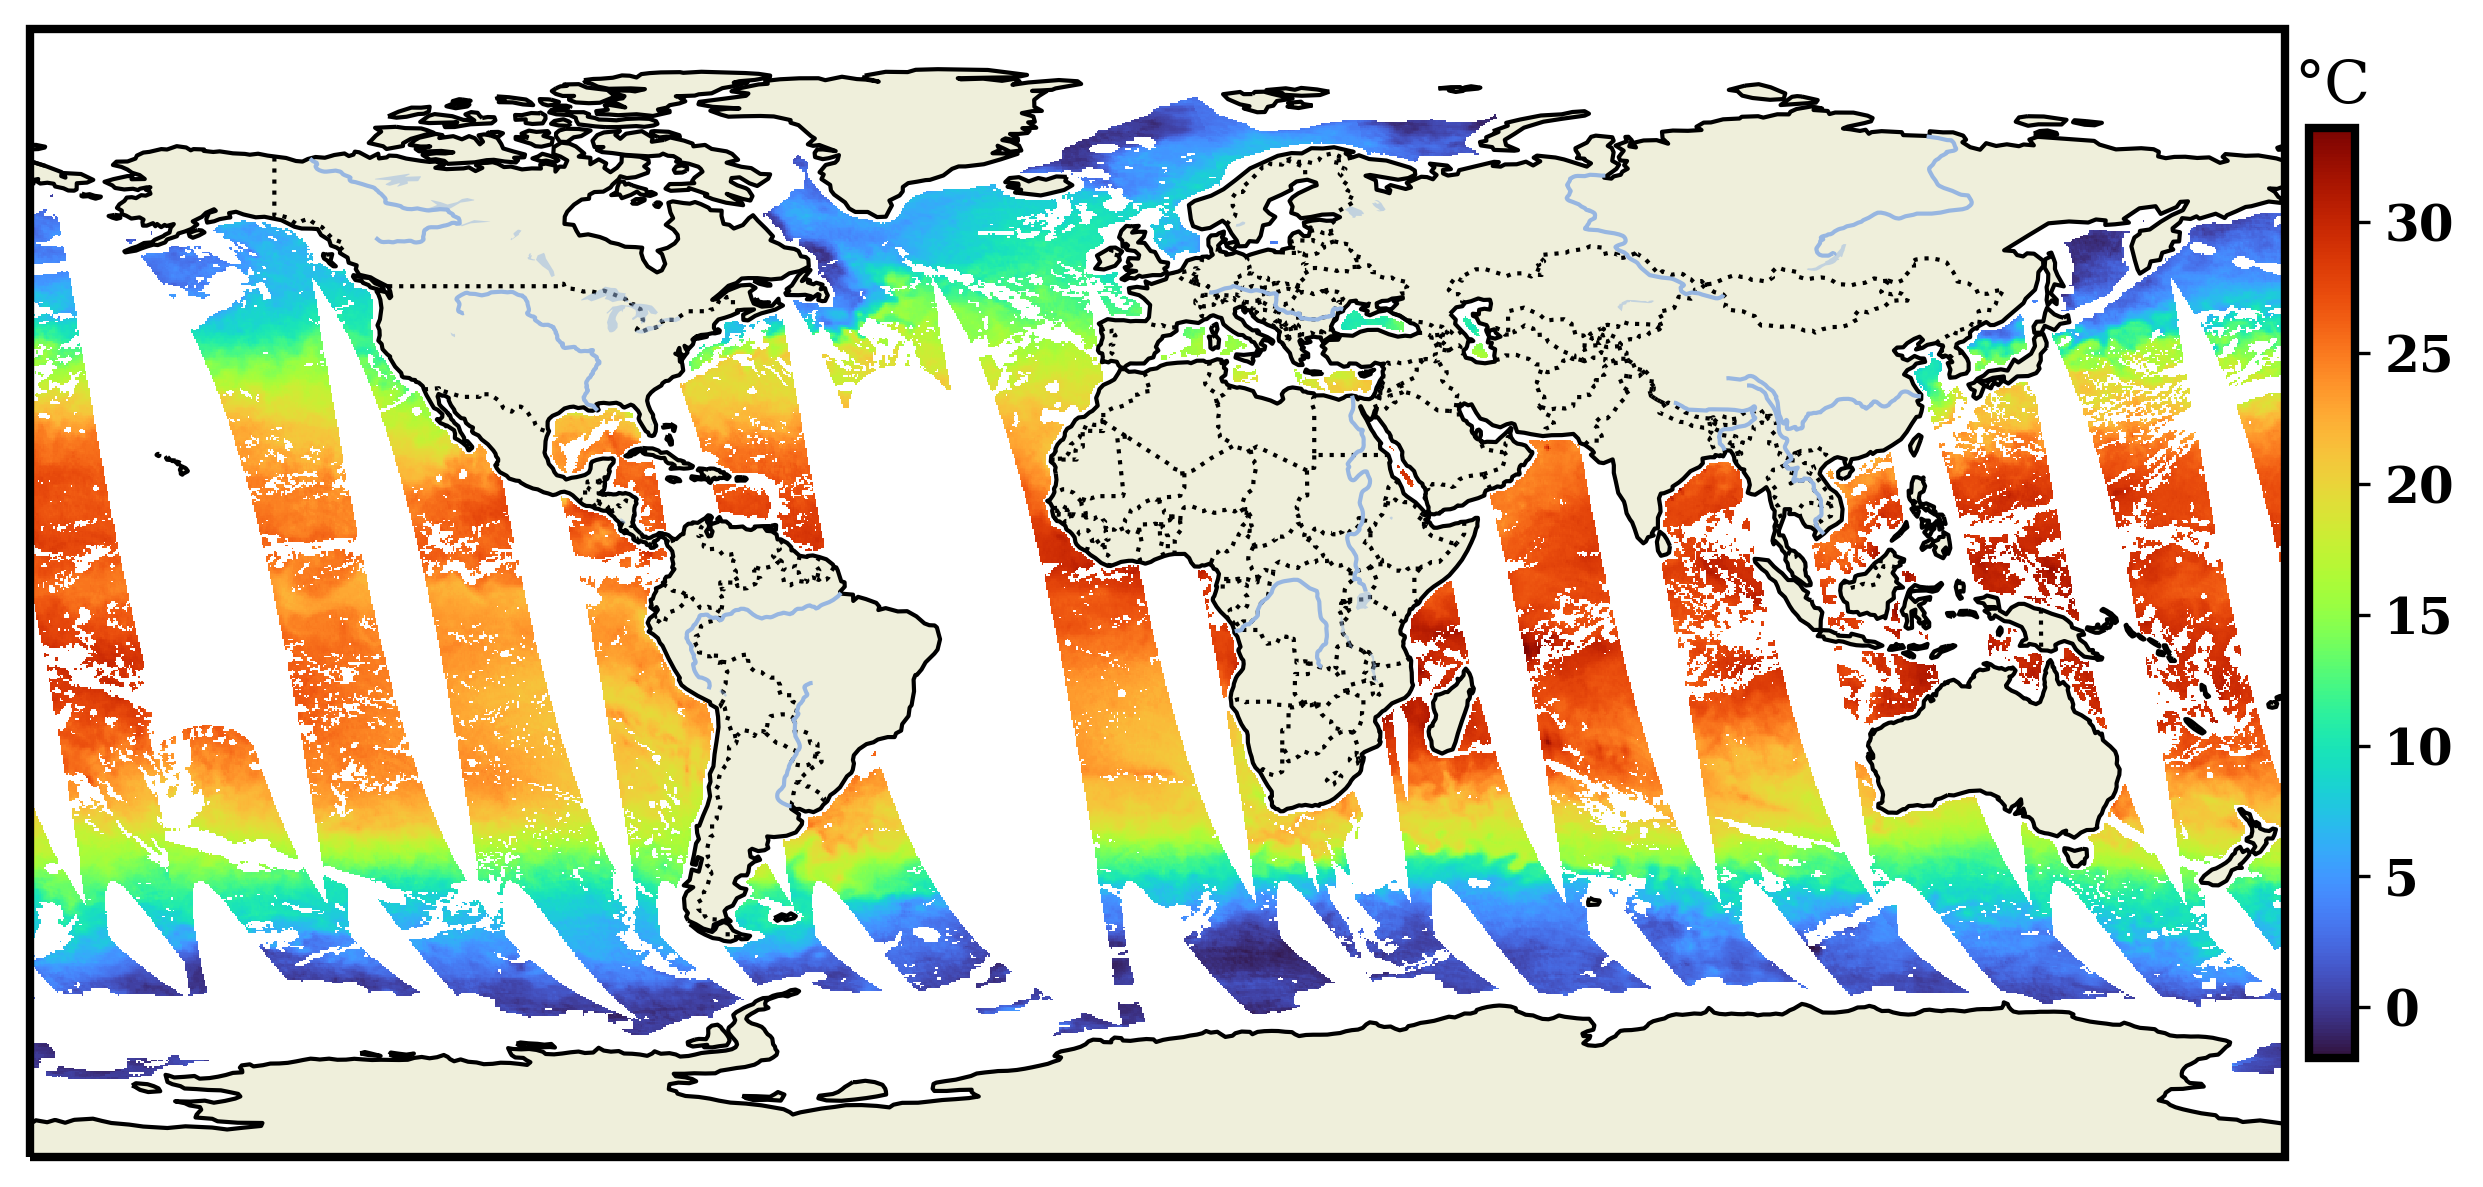
\includegraphics[width=1.0\linewidth]{m2/ims/fig2_4.png}
    \label{fig2_4}
\end{figure}

\begin{figure}[!ht]
	\centering
    \caption{L3 daily MODIS file containing only high quality flagged pixels}
	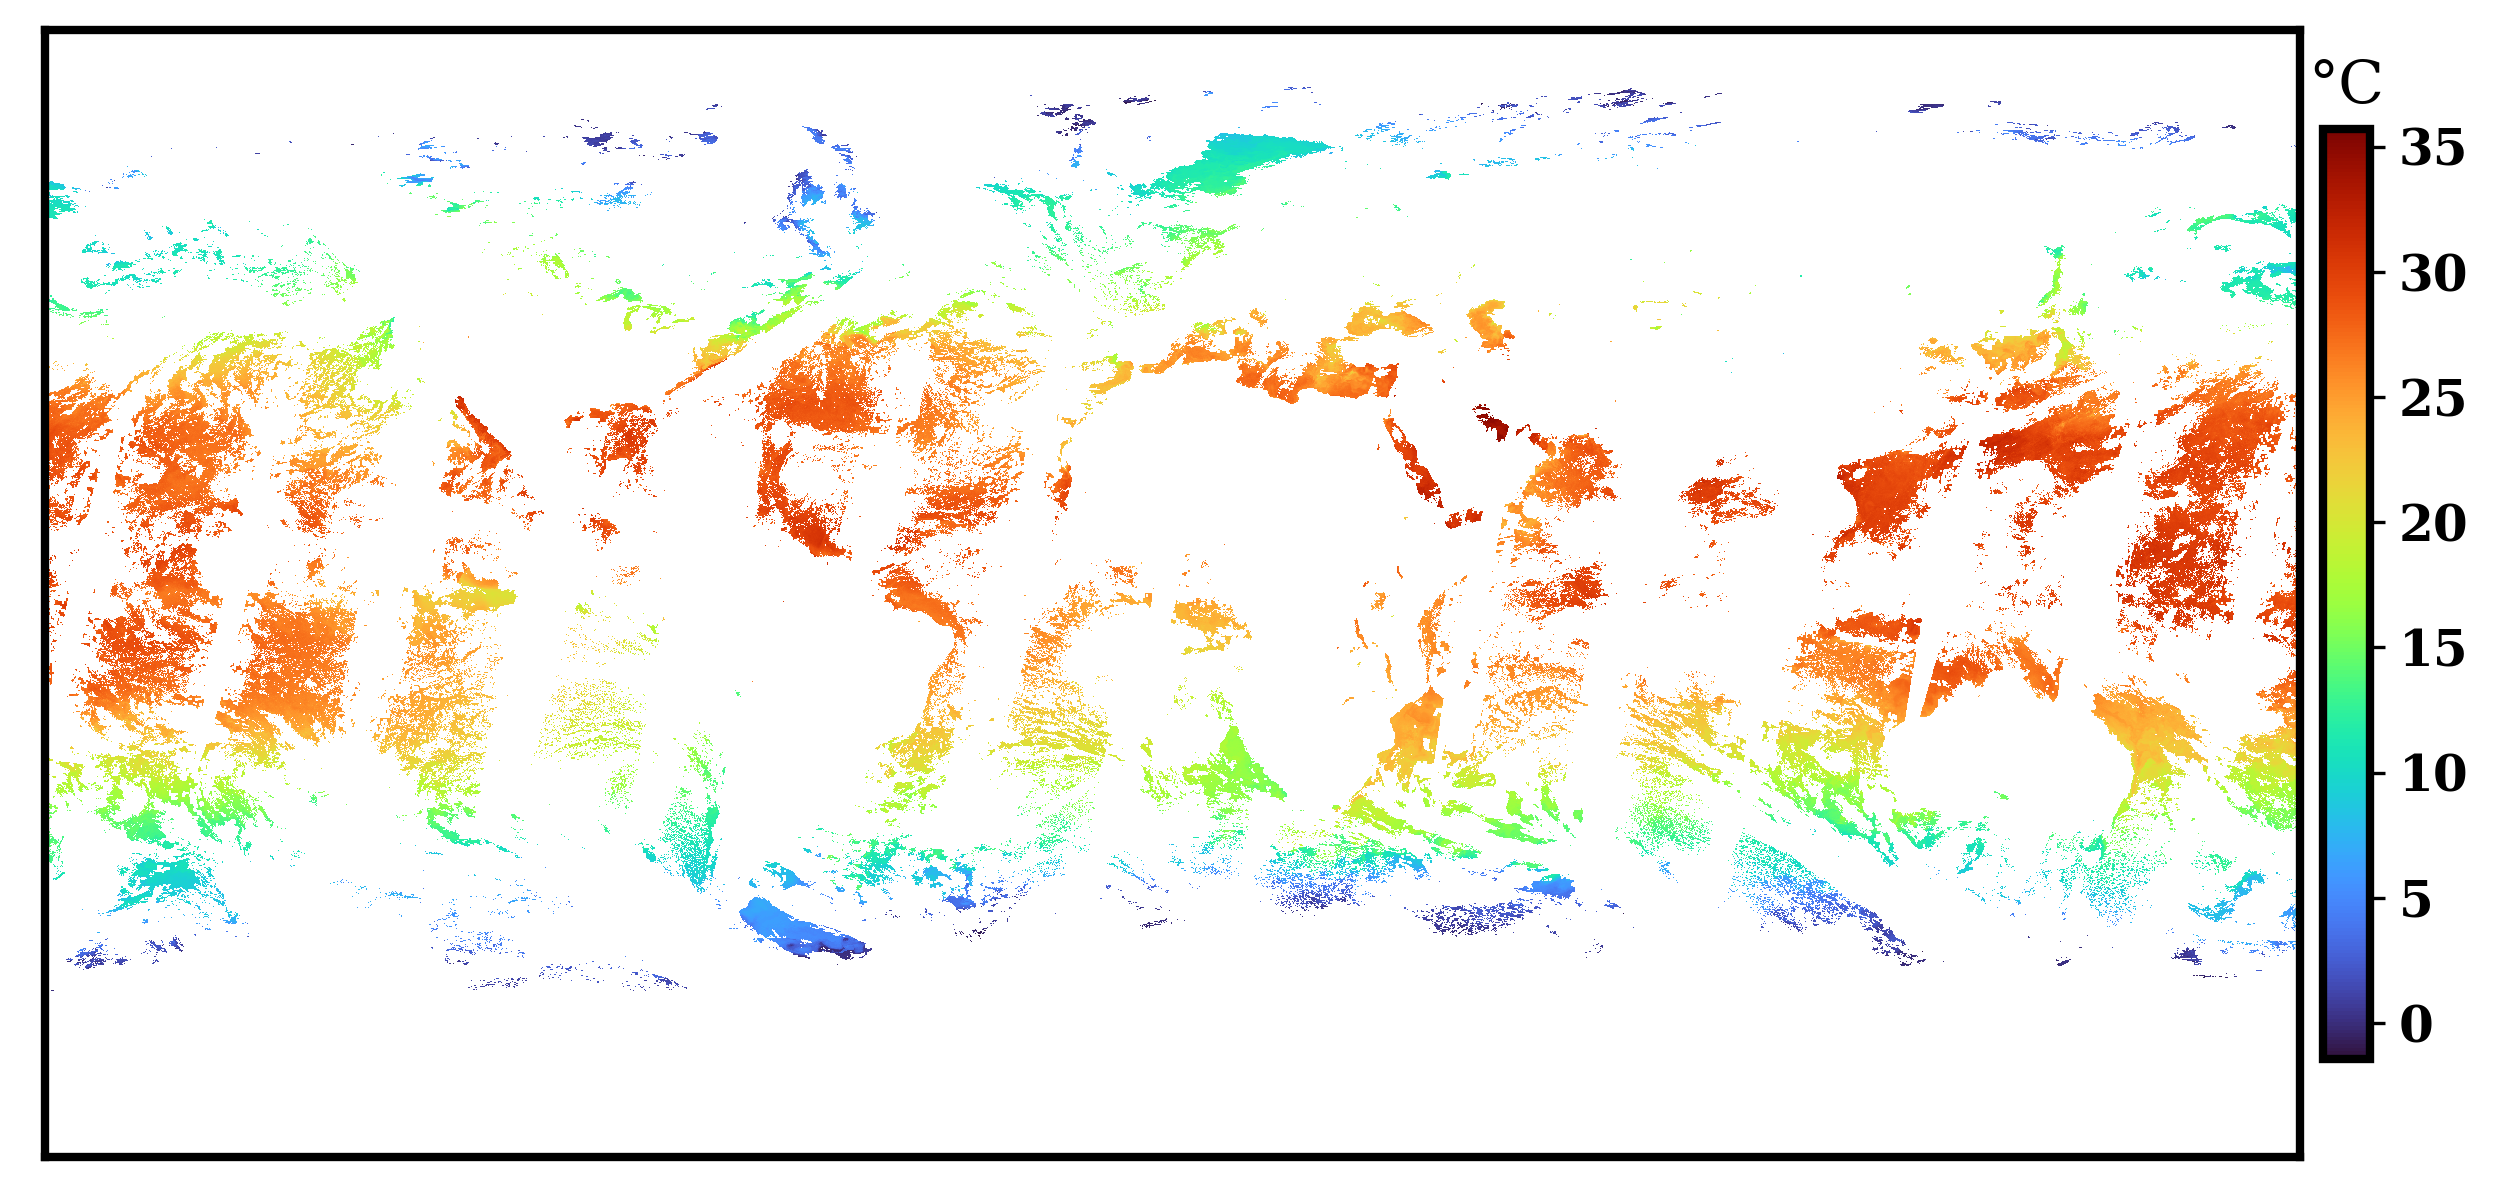
\includegraphics[width=1.0\linewidth]{m2/ims/fig2_5.png}
    \label{fig2_5}
\end{figure}

\begin{figure}[!ht]
	\centering
    \caption{Monthly L3 MODIS image containing only high quality observations}
	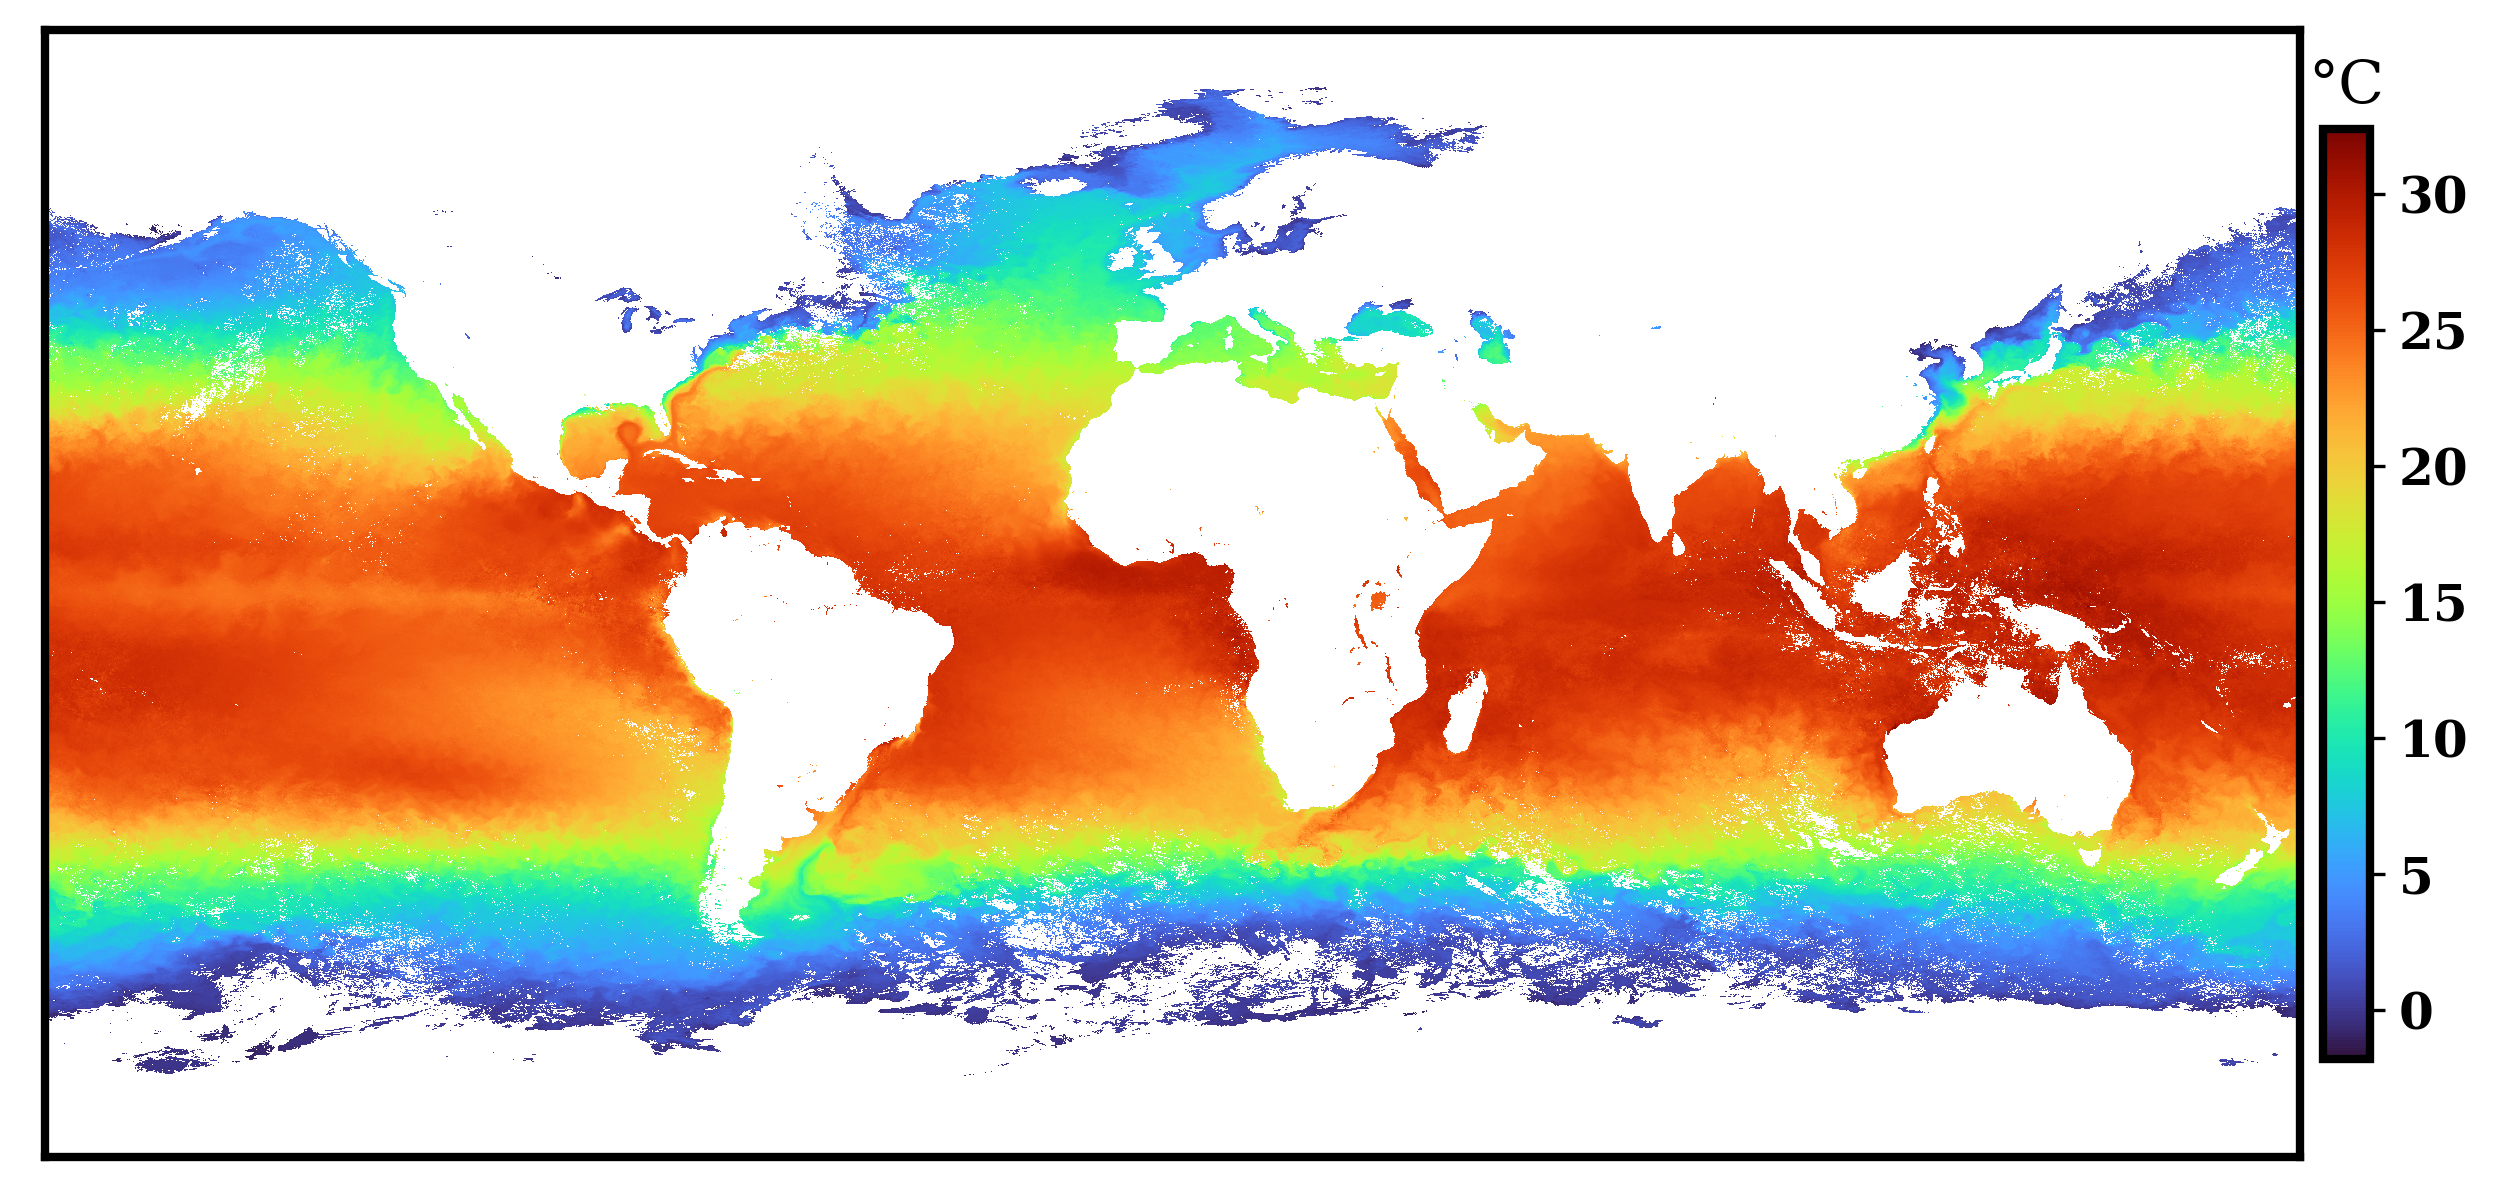
\includegraphics[width=1.0\linewidth]{m2/ims/fig2_6.png}
    \label{fig2_6}
\end{figure}

\begin{figure}[!ht]
	\centering
    \caption{Sample training monthly observation; January 2010 MODIS day observation of the Hawaiian Islands; segmented into 100 x 100 pixel regions.}
	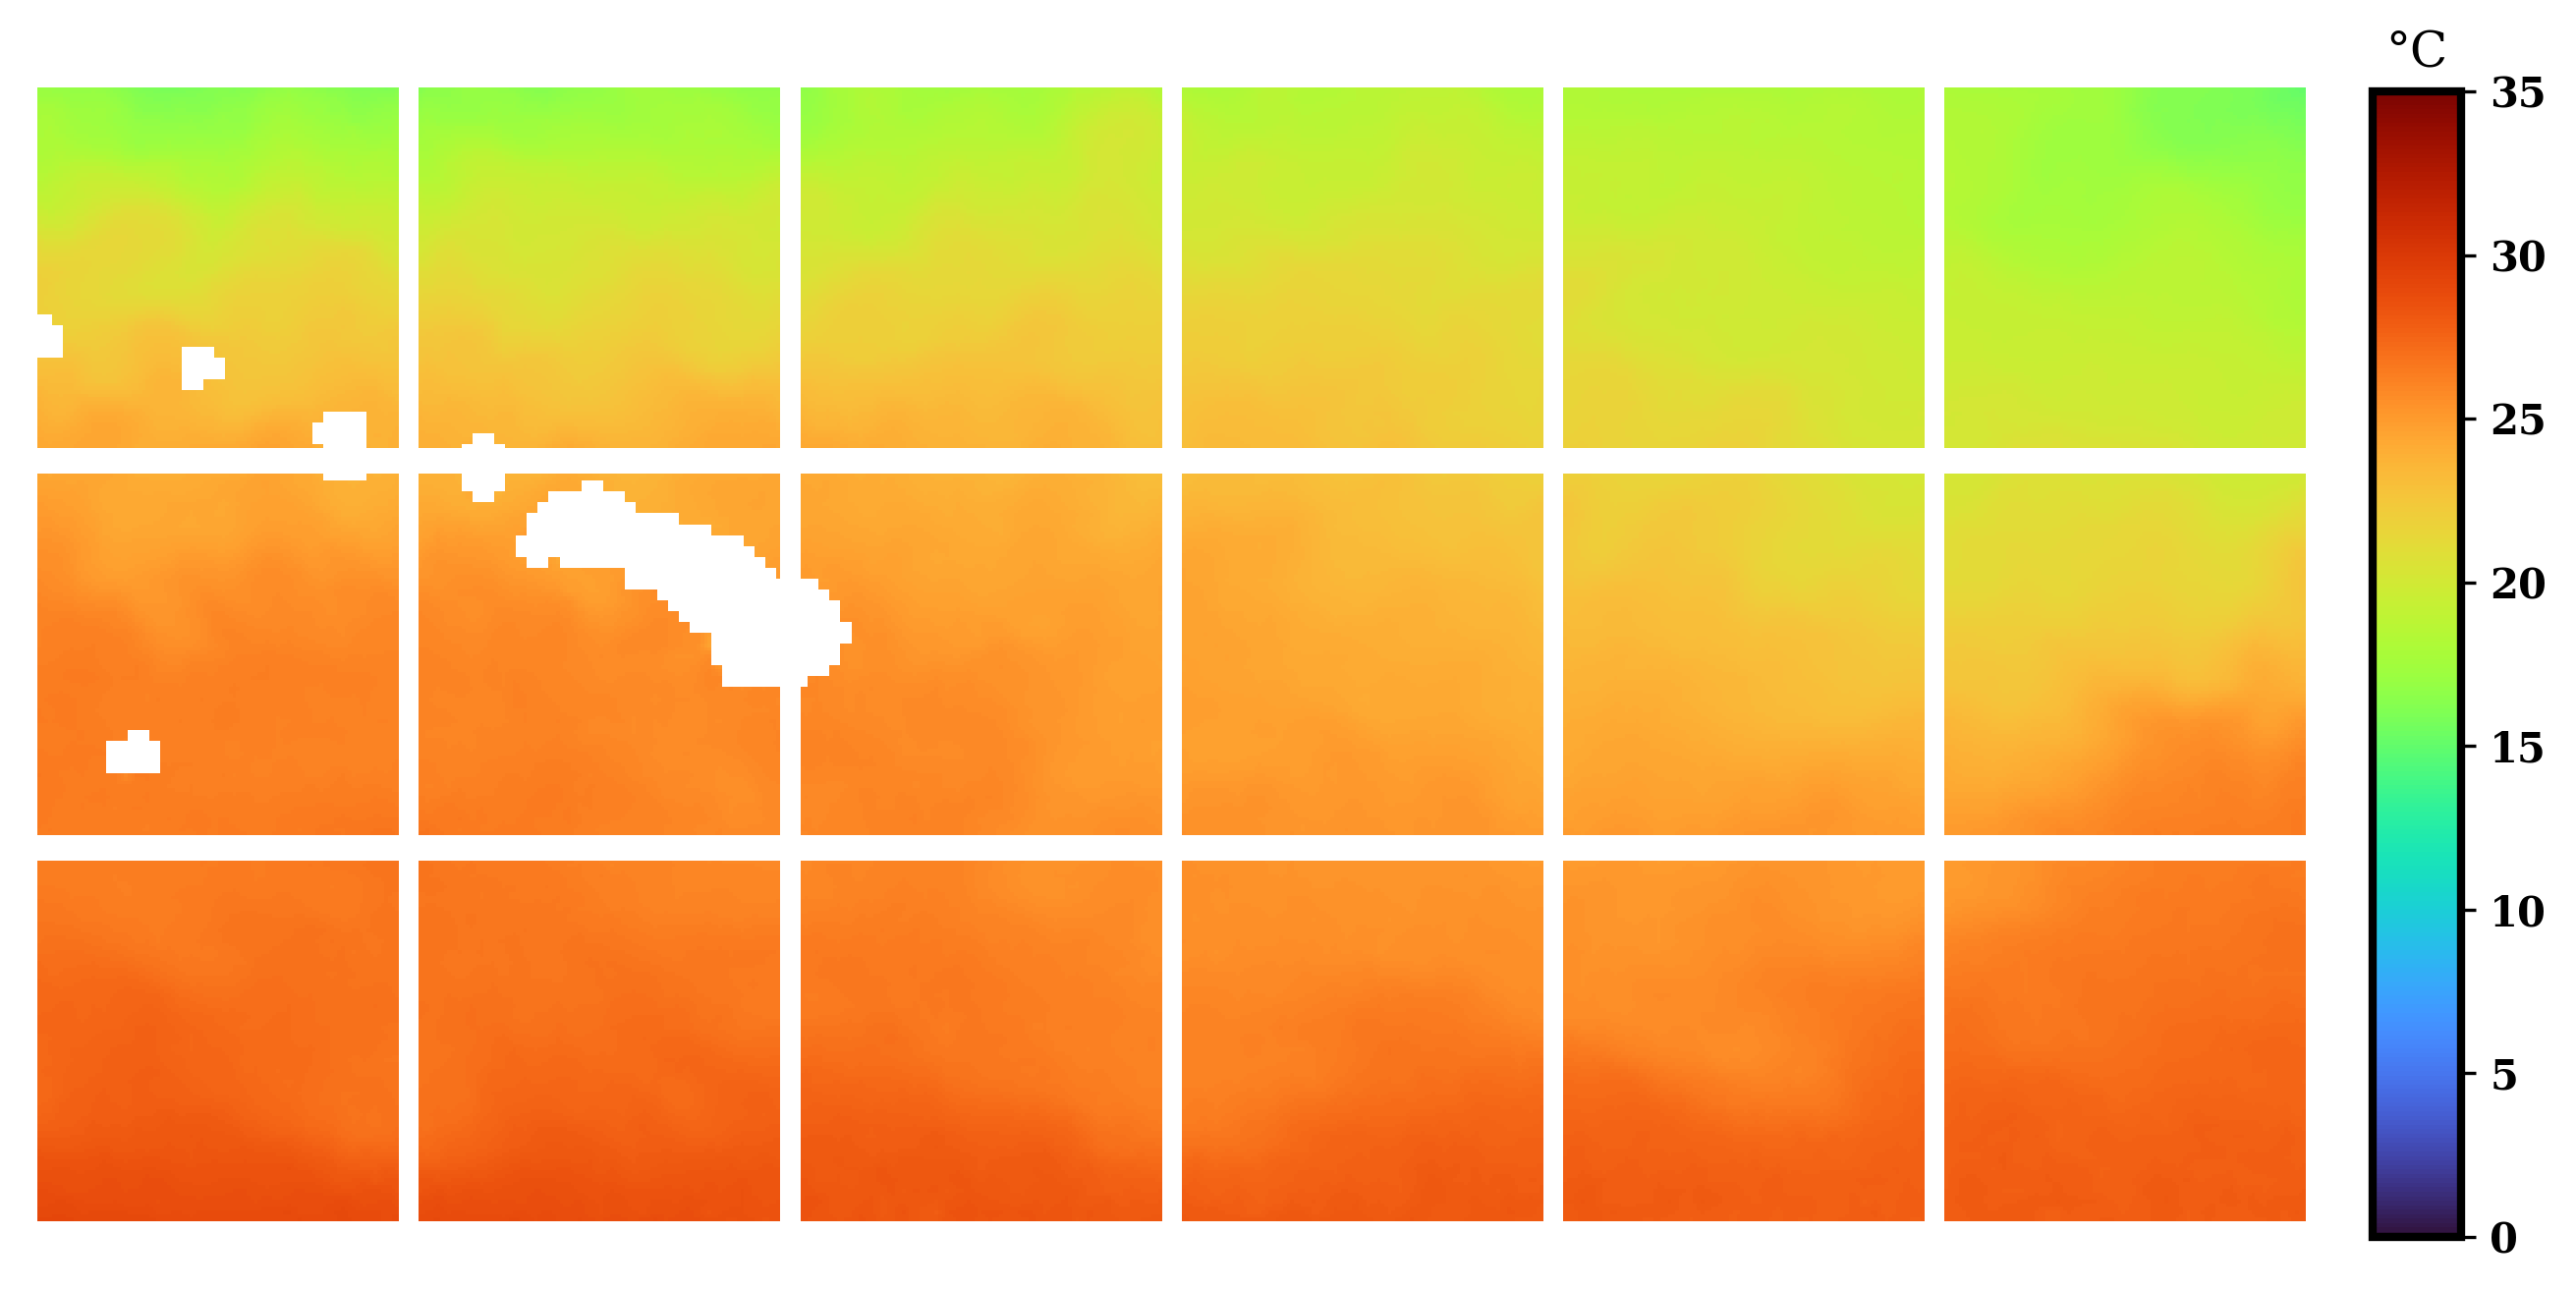
\includegraphics[width=1.0\linewidth]{m2/ims/fig2_7.png}
    
    \label{fig2_7}
\end{figure}

\begin{figure}[!ht]
	\centering
    \caption{December 2010. The top panel shows the distances from Argo and MODIS to predicted, optimized prediction, AMSR-E and each other for all nine experiments. Two bottom panels are plots of training and validation losses during neural network training.}
	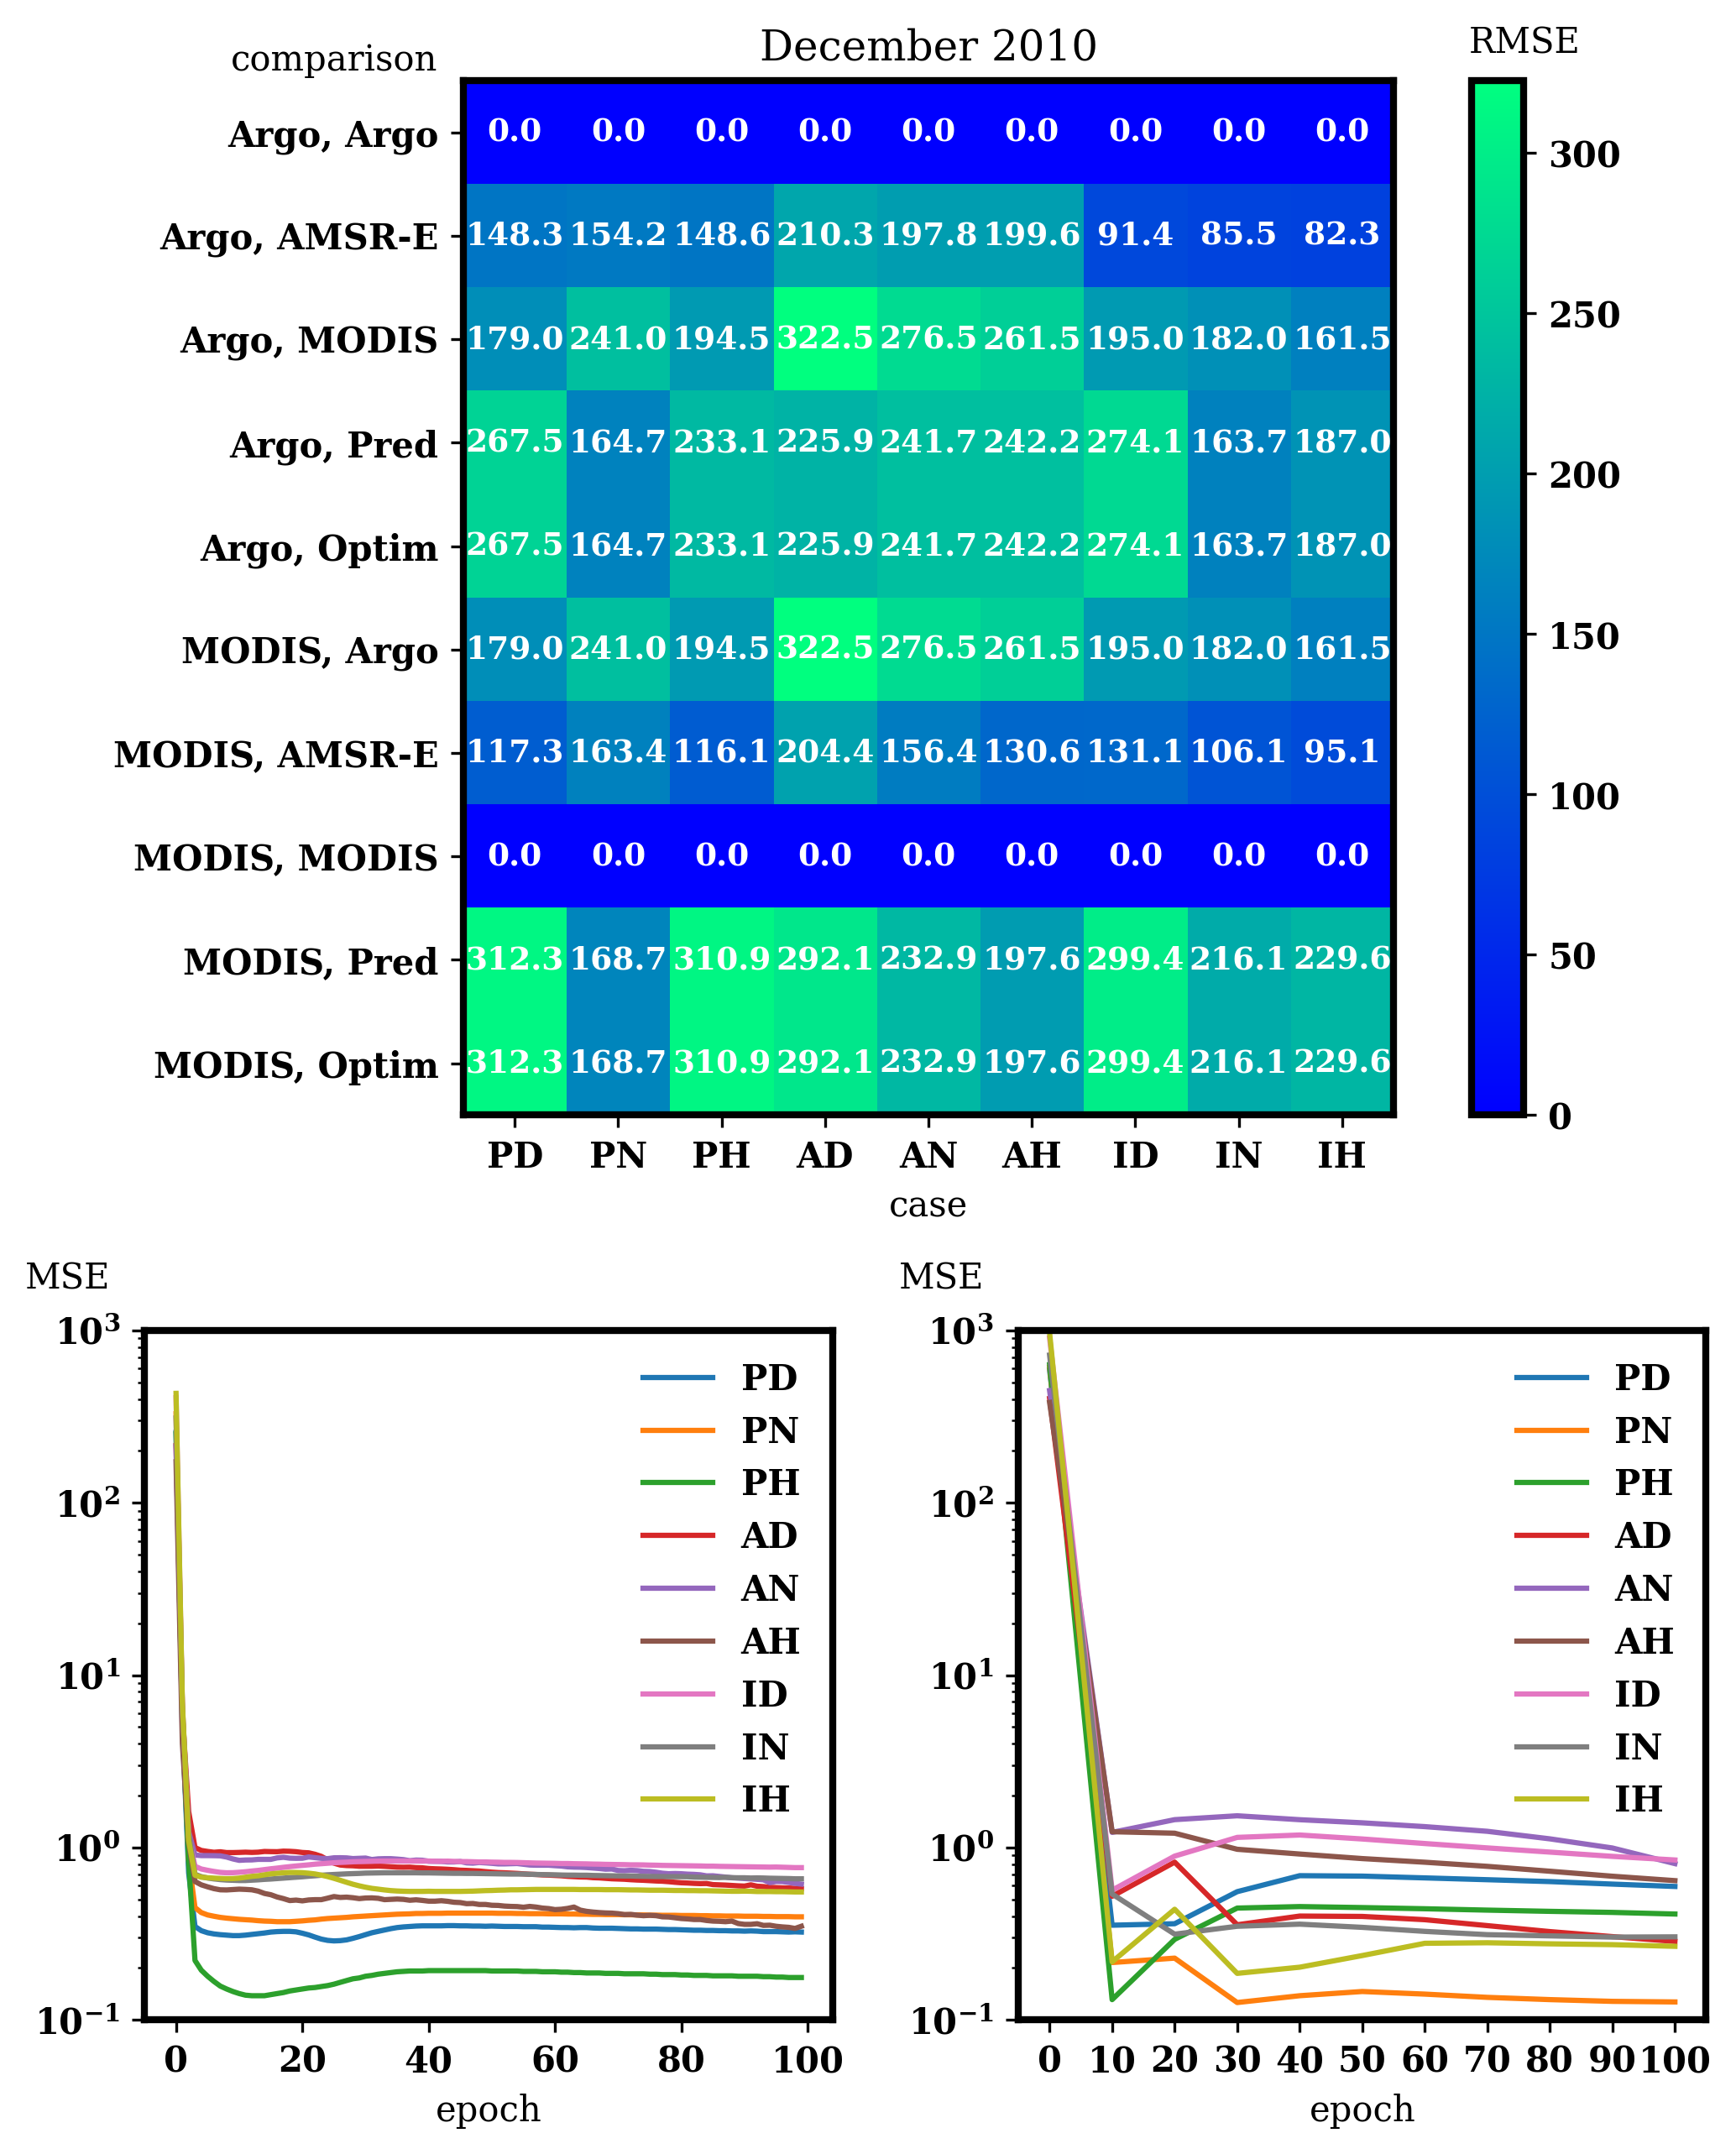
\includegraphics[width=1.0\linewidth]{m2/ims/fig2_8.png}
    \label{fig2_8}
\end{figure}

\begin{figure}[!ht]
	\centering
    \caption{Relatively “good” perceptual change, Pacific Night case}
	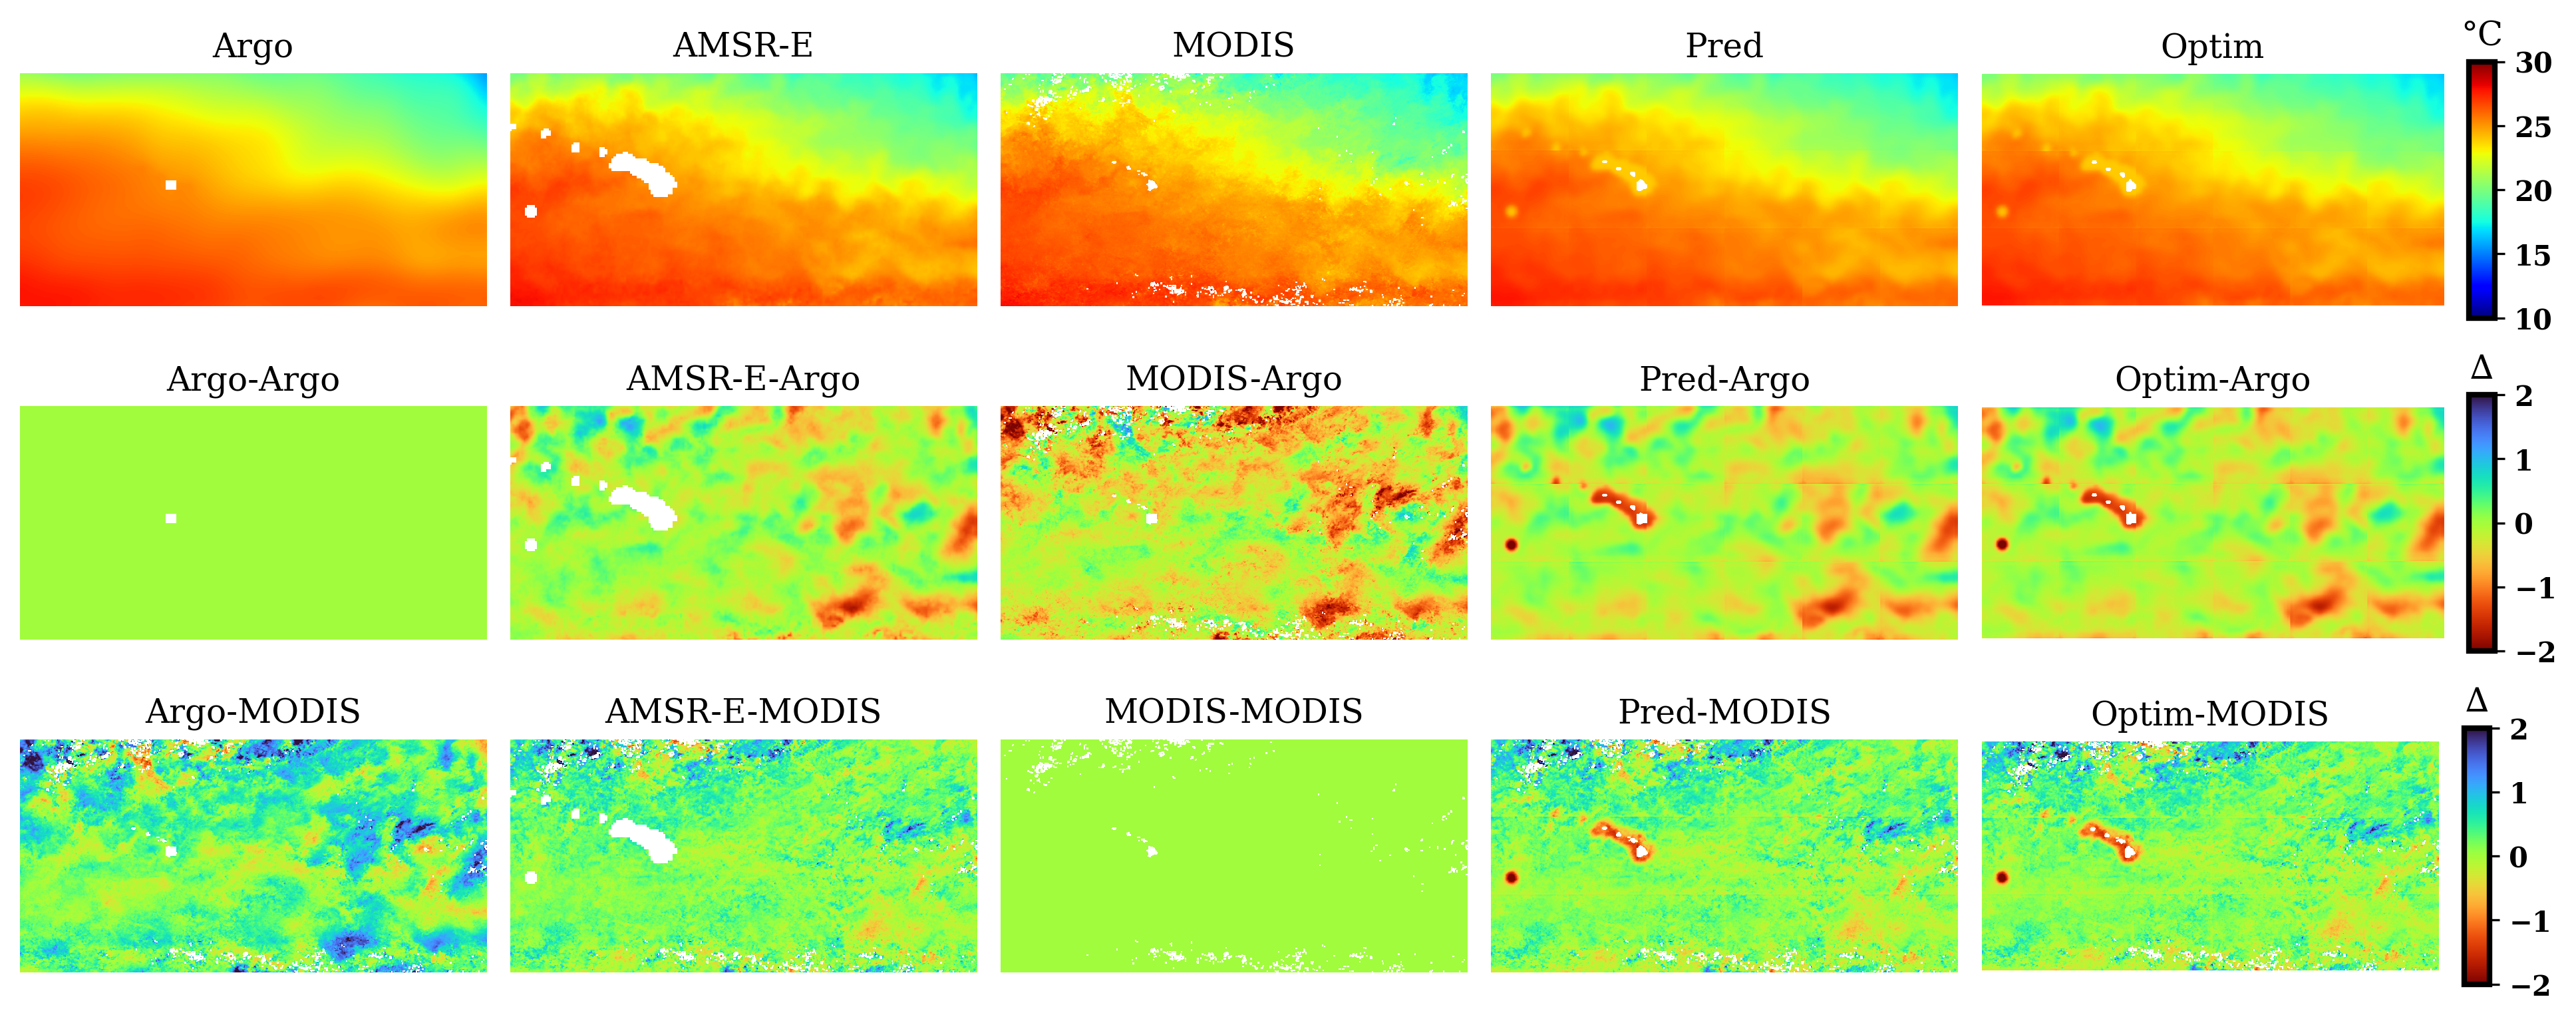
\includegraphics[width=1.0\linewidth]{m2/ims/fig2_9.png}
    \label{fig2_9}
\end{figure}


\begin{figure}[!ht]
	\centering
    \caption{Relatively “poor” perceptual change, Indian Day case}
	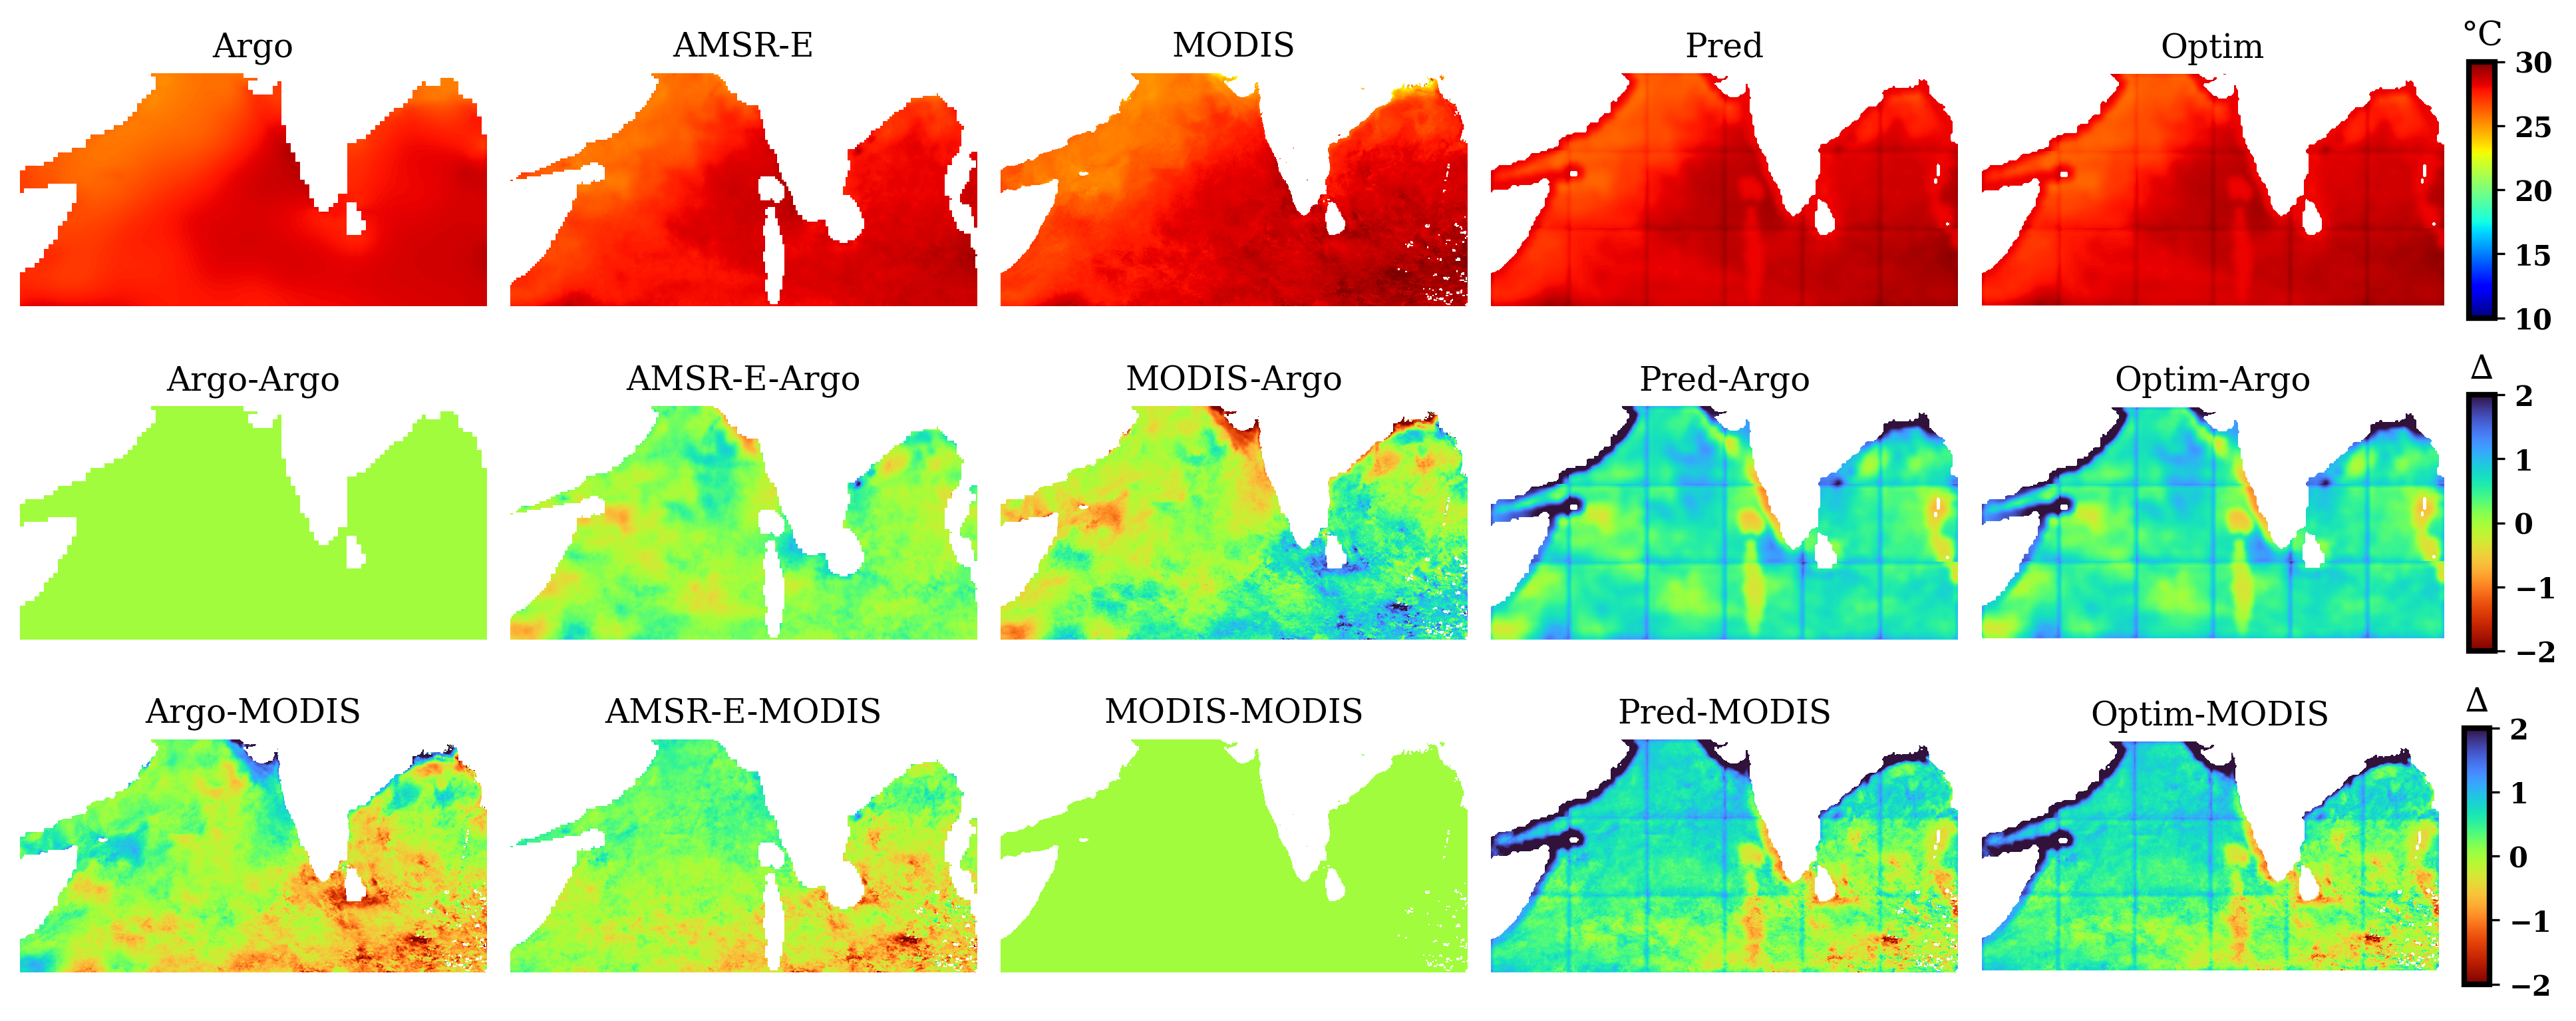
\includegraphics[width=1.0\linewidth]{m2/ims/fig2_10.png}
    \label{fig2_10}
\end{figure}

